\documentclass[ALICE,manyauthors]{ALICE_analysis_notes}
%\documentclass[ALICE,manyauthors]{ALICE_scientific_notes}
%
\usepackage{lineno}
\usepackage{xspace}
\usepackage{hyperref}
\usepackage{rotating}
\usepackage{fancyhdr}
\usepackage{amsmath}
\usepackage{graphicx}
\usepackage{verbatim}
\usepackage{amsfonts}
\usepackage{makeidx}
\usepackage{color}
\usepackage{color}
\pagestyle{headings}
\usepackage{epstopdf}
\usepackage[normalem]{ulem}
\usepackage{afterpage}
\usepackage{tabularx,booktabs}
\usepackage{multirow}
\usepackage{lineno}
\usepackage{hyperref} 
\usepackage{enumitem}
\usepackage{braket}
\usepackage{here}
\usepackage[utf8]{inputenc}
\usepackage[noadjust]{cite}

\setlist[description]{%
  topsep=5pt,               % space before start / after end of list
  itemsep=5pt,               % space between items
  %font={\bfseries\sffamily}, % set the label font
  font={\bfseries\sffamily\color{blue}}, % if colour is needed
  before={\color{blue!60!red}\itshape}
}

%%%
%%%  Alias
%%%

\makeatletter
    \setlength\@fptop{0\p@}
\makeatother

\usepackage{xspace}
\usepackage{color}
\usepackage{xcolor}
\usepackage{rotating}
\definecolor{light-gray}{gray}{0.8}

%\newcommand{\jpsi}{\rm J/$\psi$}
%\newcommand{\psip}{$\psi^\prime$}
%\newcommand{\jpsiDY}{\rm J/$\psi$\,/\,DY}
%\newcommand{\dd}{\mathrm{d}}
%\newcommand{\chic}{$\chi_{\rm c}$}
%\newcommand{\ezdc}{$E_{\rm ZDC}$}
%\newcommand{\red}{\textcolor{red}}
%\newcommand{\blue}{\textcolor{blue}}
\newcommand{\pp}{\ensuremath{\rm pp}\xspace}
\newcommand{\pPb}{p--Pb\xspace}
\newcommand{\PbPb}{Pb--Pb\xspace}
\newcommand{\AuAu}{Au--Au\xspace}
\newcommand{\ppbar}{\ensuremath{\rm p\bar{p}}\xspace}
\newcommand{\epluseminus}{\ensuremath{\rm e^{+}e^{-}}\xspace}
\newcommand{\ep}{\ensuremath{\rm ep}\xspace}

\newcommand{\MeVc}{\ensuremath{{\rm MeV/}c}\xspace}
\newcommand{\MeVcsq}{\ensuremath{{\rm MeV/}c^{2}}\xspace}
\newcommand{\GeVc}{\ensuremath{{\rm GeV/}c}\xspace}
\newcommand{\GeVcsq}{\ensuremath{{\rm GeV/}c^{2}}\xspace}
\newcommand{\eV}{\ensuremath{\rm eV}\xspace}
\newcommand{\keV}{\ensuremath{\rm keV}\xspace}
\newcommand{\MeV}{\ensuremath{\rm MeV}\xspace}
\newcommand{\GeV}{\ensuremath{\rm GeV}\xspace}
\newcommand{\TeV}{\ensuremath{\rm TeV}\xspace}
\newcommand{\fm}{\ensuremath{\rm fm}\xspace}
\newcommand{\mm}{\ensuremath{\rm mm}\xspace}
\newcommand{\cm}{\ensuremath{\rm cm}\xspace}
\newcommand{\m}{\ensuremath{\rm m}\xspace}
\newcommand{\mum}{\ensuremath{\mu{\rm m}}\xspace}
\newcommand{\s}{\ensuremath{\rm s}\xspace}
\renewcommand{\d}{\ensuremath{\rm d}\xspace}
\newcommand{\ns}{\ensuremath{\rm ns}\xspace}
\newcommand{\ps}{\ensuremath{\rm ps}\xspace}
\newcommand{\mrad}{\ensuremath{\rm mrad}\xspace}
\newcommand{\mb}{\ensuremath{\rm mb}\xspace}
\newcommand{\ctau}{\ensuremath{{\rm c}\tau}\xspace}
\newcommand{\ctauapprox}[1]{\ctau $\approx$ #1 \mum}

\newcommand{\sqrts}{\ensuremath{\sqrt{s}}\xspace}
\newcommand{\compp}{{\ensuremath{\sqrt{s}} = 7 TeV}\xspace}
\newcommand{\compPb}{{\ensuremath{\sqrt{s}} = 8.16 TeV}\xspace}
\newcommand{\sqrtsNN}{\ensuremath{\sqrt{s_{\rm NN}}}\xspace}
\newcommand{\pt}{\ensuremath{{\it p}_{\rm T}}\xspace}
\newcommand{\come}[1]{{\ensuremath{\sqrt{s}} =  #1 TeV}\xspace}
\newcommand{\comeNN}[1]{{\sqrtsNN  =  #1 TeV}\xspace}

\newcommand{\nch}{\ensuremath{N_{\rm ch}}\xspace}
\newcommand{\ntracklets}{\ensuremath{N_{\rm tracklets}}\xspace}
\newcommand{\ntrackletscorr}{\ensuremath{N^{\rm corr}_{\rm tracklets}}\xspace}
\newcommand{\dnchdeta}{\ensuremath{{\rm d}N_{\rm ch}/{\rm d}\eta}\xspace}
\newcommand{\dnchdpt}{\ensuremath{{\rm d}N_{\rm ch}/{\rm d}\pt}\xspace}
\newcommand{\dnchdy}{\ensuremath{{\rm d}N_{\rm ch}/{\rm d}y}\xspace}
\newcommand{\dntrackletsdeta}{\ensuremath{{\rm d}N_{\rm tracklets}/{\rm d}\eta}\xspace}
\newcommand{\avgntracklets}{\ensuremath{<N_{\rm tracklets}>}\xspace}
\newcommand{\avgntrackletscorr}{\ensuremath{<N^{\rm corr}_{\rm tracklets}>}\xspace}
\newcommand{\dnhfedeta}{\ensuremath{{\rm d}N_{\rm HFE}/{\rm d}\eta}\xspace}
\newcommand{\dndeta}{\ensuremath{{\rm d}N/{\rm d}\eta}\xspace}

\newcommand{\ptmore}[1]{{\pt $>$ #1 \GeVc}\xspace}
\newcommand{\ptless}[1]{{\pt $<$ #1 \GeVc}\xspace}
\newcommand{\ptrange}[2]{{#1 $<$ \pt $<$ #2  \GeVc}\xspace}
\newcommand{\etaless}[1]{\ensuremath{\left|\eta\right| < #1}\xspace}
\newcommand{\etarange}[2]{\ensuremath{#1 < \eta < #2}\xspace}
\newcommand{\yless}[1]{\ensuremath{\left|y\right| < #1}\xspace}
\newcommand{\yfid}{\ensuremath{y_{\rm fid}(\pt)}\xspace}
\newcommand{\yfidcut}{\ensuremath{\left|y\right| < y_{\rm fid}(\pt)}\xspace}
\newcommand{\dnchdetaless}[1]{\ensuremath{{\rm d}N_{\rm ch}/{\rm d}\eta|_{\etaless{#1}}}\xspace}
\newcommand{\zvertex}{\ensuremath{z_{\rm vtx}}\xspace}
\newcommand{\zvertexless}[1]{\ensuremath{\left|z_{\rm vtx}\right| < #1\ \cm}\xspace}
\newcommand{\zvertexout}[1]{\ensuremath{\left|z_{\rm vtx}\right| > #1\ \cm}\xspace}

\newcommand{\slfrac}[2]{\ensuremath{\left.#1\right/#2}\xspace}
\newcommand{\dedx}{\ensuremath{{\rm d}E/{\rm d}x}\xspace}
\newcommand{\asymmerr}[2]{\ensuremath{^{+#1}_{-#2}}\xspace}
\newcommand{\average}[1]{\ensuremath{\langle #1 \rangle}\xspace}
\newcommand{\nluminosity}[2]{\ensuremath{L_\text{int} = {#1}\pm{#2}\ \text{nb}^{-1}}\xspace}
\newcommand{\luminosity}{\ensuremath{L_\text{int}}\xspace}

\newcommand{\sphero}{\ensuremath{{S}_{\textit O}}\xspace}
\newcommand{\Dzero}{\ensuremath{{\rm D}^{0}}\xspace}
\newcommand{\Dzerobar}{\ensuremath{\overline{{\rm D}^{0}}}\xspace}
\newcommand{\DzeroNS}{\ensuremath{{\rm D}^{0}}}       %NS = No space
\newcommand{\Dstarplus}{\ensuremath{{\rm D}^{*+}}\xspace}
\newcommand{\DstarplusNS}{\ensuremath{{\rm D}^{*+}}}       %NS = No space
\newcommand{\Dplus}{\ensuremath{{\rm D}^{+}}\xspace}
\newcommand{\DplusNS}{\ensuremath{{\rm D}^{+}}}       %NS = No space
\newcommand{\Piplus}{\ensuremath{{\pi}^{+}}\xspace}
\newcommand{\PiplusNS}{\ensuremath{{\pi}^{+}}}        %NS = No space
\newcommand{\Piminus}{\ensuremath{{\pi}^{-}}\xspace}
\newcommand{\PiminusNS}{\ensuremath{{\pi}^{-}}}
\newcommand{\sPi}{\ensuremath{{\pi}}\xspace}
\newcommand{\Kplus}{\ensuremath{{\rm K}^{+}}\xspace}
\newcommand{\KplusNS}{\ensuremath{{\rm K}^{+}}}
\newcommand{\Kminus}{\ensuremath{{\rm K}^{-}}\xspace}
\newcommand{\KminusNS}{\ensuremath{{\rm K}^{-}}}
\newcommand{\sProton}{\ensuremath{\rm p}\xspace}
\newcommand{\pProtonNS}{\ensuremath{\rm p}}
\newcommand{\apProton}{\ensuremath{\overline{\rm p}}\xspace}
\newcommand{\apProtonNS}{\ensuremath{\overline{\rm p}}}
\newcommand{\sKzero}{\ensuremath{2{\rm K}^{0}_{S}}\xspace}
\newcommand{\pKzero}{\ensuremath{{\rm K}^{0}_{S}}\xspace}
\newcommand{\sXi}{\ensuremath{\Xi}\xspace}
\newcommand{\pXi}{\ensuremath{\Xi^{-}}\xspace}
\newcommand{\pXiNS}{\ensuremath{\Xi^{-}}}
\newcommand{\apXi}{\ensuremath{\overline{\Xi}^{+}}\xspace}
\newcommand{\apXiNS}{\ensuremath{\overline{\Xi}^{+}}}
\newcommand{\Jpsi}{\ensuremath{{\rm J}/\psi}\xspace}

\newcommand{\DtoKpi}{\ensuremath{{\Dzero}\to{\KminusNS}{\PiplusNS}}\xspace} 
\newcommand{\DbartoKpi}{\ensuremath{{\Dzerobar}\to{\KplusNS}{\PiminusNS}}\xspace}   
\newcommand{\DtoKpipi}{\ensuremath{{\Dplus}\to{\KminusNS}{\PiplusNS}{\PiplusNS}}\xspace}   
\newcommand{\DstartoDpi}{\ensuremath{{\Dstarplus}\to{\DzeroNS}{\PiplusNS}}\xspace}   

\newcommand{\brDtoKpi}{\ensuremath{{\rm 3.93} \pm {\rm 0.04}\%}\xspace}   
\newcommand{\brDtoKpipi}{\ensuremath{{\rm 9.46} \pm {\rm 0.24}\%}\xspace}   

\newcommand{\error}[1]{{\color{red}\bf \textsc{Wrong:} #1}}
\newcommand{\warning}[1]{{\color{red}\bf \textsc{Warning:} #1}}
\newcommand{\comments}[1]{{\color{blue}\bf \textsc{Comment:} #1}}
\newcommand{\correct}[2]{{\color{red}\sout{#1}}{\color{blue}\xspace#2}}
\newcommand{\cmnt}[1]{}
\newcommand{\fake}[1]{{\color{red}\bf#1}}

\newcommand{\alphas}{\ensuremath{\alpha_{\rm S}}\xspace}
\newcommand{\SPS}{\ensuremath{\rm Sp\bar{p}S}\xspace}
\newcommand{\Raa}{\ensuremath{R_{\rm AA}}\xspace}
\newcommand{\Rppb}{\ensuremath{R_{\rm pPb}}\xspace}
\newcommand{\Rpa}{\ensuremath{R_{\rm pPb}}\xspace}

%%%
%%% end Alias
%%%

\linenumbers

%%%%%%%%%%%%%%%%%%%%%%%%%%%%%%%%%%%%%%%%%%%%%
%\usepackage[backend=biber,backref=false,
%sorting=none,style=numeric,
%isbn=false,doi=false,hyperref=true,
%url=false,eprint=true,firstinits=true]{biblatex}
%%%%% you can add multiple bib files containing your refrences %%%%%%%%%%%%
%\addbibresource{refer.bib}
%%%%%%%%%%%%%%%%%%%%%%%%%%%%%%%%%%%%%%%%%%%%%

%\usepackage[square,numbers,sort&compress]{natbib}

\begin{document}
%%%%%%%%%%%%% ptdr definitions %%%%%%%%%%%%%%%%%%%%%
%%%%%%%%%%%%%%%  Title page %%%%%%%%%%%%%%%%%%%%%%%%
%

\begin{titlepage}
%
\PHnumber{ALICE-2020-xxx} 
\PHdate{\today}
%
%%% Put your own title + short title here:
\title{ Inclusive and multiplicity dependent production of electrons from heavy-flavour hadron decays in pp and \pPb collisions}
%\ShortTitle{}   
\ShortTitle{electrons from heavy-flavour hadron decays in pp and \pPb collisions.}
% appears on right page headers
%
%\author{Authors list to be filled}
%\Collaboration{ Authors list to be filled }%
\author{ALICE Collaboration$^{*}$}
\ShortAuthor{ALICE Analysis Note 2017} % appears on left page headers, do not change
%
\begin{abstract}

Heavy-flavour production at midrapidity is studied using electrons from heavy-flavour hadron decays in pp collisions at $\sqrt{s}=13$ TeV to precisely test perturbative QCD calculations, and to study effects from cold nuclear matter (CNM) in \pPb collisions at $\sqrt{s_{\rm{NN}}} = 8.16$ TeV. Furthermore, their production in-terms of self-normalized yield as a function of normalized charged-particle multiplicity, estimated at midrapidity, in pp and \pPb collisions is studied to investigate the role of multiple-parton interactions (MPI) and the interplay between hard and soft mechanism in particle production. The production cross section of electrons from heavy-flavour hadron decays measured in the transverse momentum (\pt) range from $0.2$ $< p_{\rm T} <$ $35$ GeV$/c$ in pp collisions at $\sqrt{s}=13$ TeV is compared with pQCD calculation. The nuclear modification factor of electrons from heavy-flavour hadron decays measured as a function of \pt in \pPb collisions at $\sqrt{s_{\rm{NN}}} = 8.16$ TeV in the range 0.5 $< p_{\rm T} <$ 26 GeV/$c$, is consistent with unity within the statistical and systematic uncertainties. The self-normalized yield in pp and \pPb collisions grows faster than linear with the normalized multiplicity. In pp collisions a strong \pt dependence is observed, where the yield of higher \pt electrons increases faster as a function of multiplicity compared to the one of lower \pt electron. The measurement in \pPb collisions shows a weaker \pt dependence within uncertainties. The self-normalized yield in pp collisions is compared with PYTHIA 8.2 Monte-Carlo simulations and with measurements of inclusive charged particles, D-mesons and J/$\psi$. In \pPb collisions, the self-normalized yield as a function of normalized charged-particle multiplicity is compared with D-mesons measurements. 

%Heavy-flavour production studies in pp collisions, besides providing the necessary baseline for measurements in \PbPb collisions, constitute a precision test of perturbative QCD calculations. In complex systems such as \pPb collisions, it gives insights into the cold nuclear matter (CNM) effects. Furthermore, their production as a function of charged-particle multiplicity in pp and \pPb collisions provides insights into the role of multiple-parton interactions (MPI) and the interplay between hard and soft mechanism in particle production. In \pPb collisions, the production is also influenced by the concurrent multiple binary nucleon-nucleon collisions. 
%In this paper, we will present the measurement of the yield of electrons from heavy-flavour hadron decays at midrapidity as a function of the transverse momentum and charged-particle multiplicity estimated at midrapidity (self-normalized yield) in pp collisions at \sqrts = 13 TeV and in \pPb collisions at \sqrtsNN = 8.16 \TeV.
\\
\\
{\it Keywords:} Heavy-flavour electrons, nuclear modification factor, self-normalized yield, multiplicity, pp collisions, \pPb collisions

\end{abstract}
\end{titlepage}
\section{Introduction}\label{section:introduction}
In high-energy hadronic collisions, heavy quarks, i.e charm and beauty are mainly produced in hard parton scattering processes. Due to their large masses, their production cross sections can be calculated in the framework of perturbative Quantum Chromodynamics (pQCD) down to low transverse momenta~\cite{Kniehl:2008zza,Cacciari:2003uh,Kniehl:2005mk,Cacciari:2003zu}, %making them a very important tool to study 
in hadronic collisions. In heavy-ion collisions at ultra-relativistic energies, it is well established that a strongly coupled quark gluon-plasma (QGP) is formed~\cite{Karsch:2006xs,Borsanyi:2010cj,Bazavov:2011nk}. In the presence of the QGP a suppression of the heavy-flavour particles produced in the collisions with a high transverse momentum ($p_{\textrm{T}}$) is observed ~\cite{ALICE:2012ab,Abelev:2012qh,Adam:2015nna,Adam:2016khe,Sirunyan:2017xss, Acharya:2020lgn}. 
%{\color{blue}Write a sentence about v2...}

Measurements of heavy flavour hadron production in proton-proton collisions at the Large Hadron Collider (LHC) provide a way to test pQCD calculations at the highest available collision energies and constitute a baseline for the study of heavy-flavour production in heavy-ion collisions. The inclusive production cross sections of charm mesons and their decay products measured in pp collisions at the LHC at both mid-and forward-rapidity~\cite{Abelev:2012pi,Abelev:2012vra,Abelev:2012xe,Aaij:2016jht} are described by theoretical predictions based on pQCD calculations, with the collinear factorisation approach at next-to-leading order (e.g. in the general-mass variable-flavour-number scheme, GM-VFNS~\cite{Kniehl:2008eu,Kniehl:2011bk}) or at fixed order with next-to-leading-log resummation (FONLL~\cite{Cacciari:2012ny}) within theoretical uncertainties.
%The measured D-meson production cross sections in pp collisions at the LHC can also be described by pQCD calculations performed in the framework of $k_{\textrm{T}}$-factorisation in the leading order (LO) approximation~\cite{Maciula:2013oba}. 
Beauty production cross section measurements in pp collisions at $\sqrt{s}=7$ and $2.76$ TeV~\cite{Abelev:2012gx,Adam:2016wyz,ATLAS:2013cia,Khachatryan:2010yr,Aaij:2010gn}  are well described by implementations of FONLL and GM-VFNS~\cite{Cacciari:2012ny,Kniehl:2005ej,Maciula:2013wg,Abelev:2012gx,Abelev:2012sca,ATLAS:2013cia,Khachatryan:2010yr,Aaij:2010gn,Kniehl:2011bk}. 
%{\color{blue}Include HFE as well??}

In proton-nucleus collisions, the so-called ‘Cold Nuclear Matter’ (CNM) effects occur due to the presence of a nucleus in the colliding system, and, possibly, to the large density of produced particles. In particular, the parton distribution functions (PDFs) of nucleons bound in nuclei are modified with respect to those of free nucleons, which can be described by phenomenological parameterisations referred to as nuclear PDFs (nPDFs)~\cite{Eskola:2009uj,deFlorian:2003qf,Hirai:2007sx}. When the production process is dominated by gluons at low Bjorken-x, the nucleus can be described by the Colour-Glass Condensate (CGC) effective theory as a coherent and saturated gluonic system~\cite{Fujii:2013yja,Tribedy:2011aa,Albacete:2012xq,Rezaeian:2012ye}. The kinematics of the partons in the initial state can be affected by multiple scatterings 
%(transverse momentum broadening, or $k_{\textrm{T}}$ broadening)
~\cite{Lev:1983hh,Kopeliovich:2002yh} or by gluon radiation (energy loss) before or after the heavy-quark pair is produced~\cite{Vitev:2007ve}. Measurement of heavy-flavour production in \pPb collisions at the LHC will allow a study of the above mentioned effects. Previous measurements of the nuclear-modification factor of heavy-flavour hadrons and its decay leptons in \pPb collisions at $\sqrt{s_{\textrm{NN}}}=5.02$ TeV indicate no significant modification of their yields due to CNM effects in the measured  transverse momentum region within the uncertainties of the measurements~\cite{Adam:2015qda,Adam:2016wyz,Abelev:2014hha}. 


Recent measurements of light-flavour and heavy-flavour hadrons in high multiplicity pp, p-A and d-A collisions at different energies have revealed strong flow-like effects in these small systems~\cite{Acharya:2018dxy,Abelev:2012ola,Aaboud:2016yar,Chatrchyan:2013nka,ABELEV:2013wsa,Khachatryan:2014jra,Adare:2013piz,Adamczyk:2015xjc,Adare:2015ctn,Khachatryan:2010gv}. The origin of these phenomena is debated, and several models with microscopic and macroscopic approaches describe qualitatively the observed features in high multiplicity events.  While macroscopic models incorporate hydrodynamical evolution of the system~\cite{Werner:2010ss,Deng:2011at,Werner:2013ipa}, the others include overlapping strings~\cite{Bierlich:2014xba}, string percolation~\cite{Bautista:2015kwa}, multi-parton interactions and color reconnection~\cite{Sjostrand:2014zea,Ortiz:2013yxa}. A multiphase transport model~\cite{Koop:2015wea}, as well as the fragmentation of saturated gluon states~\cite{Schlichting:2016sqo,Schenke:2016lrs}, is able to describe some features of the data. The measurement of heavy-flavour production in small systems as a function of the charged-particle multiplicity produced in the collision could thus provide further insight into the processes occurring in the collision at the partonic level and the interplay between the hard and soft mechanisms in particle production in pp and \pPb collisions. 

Measurements of open and hidden charm and beauty production~\cite{Adam:2015ota,Acharya:2020pit,Adam:2018jmp,Chatrchyan:2013nza,Acharya:2020giw,Adam:2016mkz} indicate an increase of heavy-flavour production with charged-particle multiplicity measured at midrapidity. D-meson~\cite{Adam:2015ota} and J$/\psi$~\cite{Acharya:2020pit,Adam:2018jmp} production normalized to their corresponding averages in minimum bias events, measured as a function of normalized event multiplicities in pp collisions $\sqrt{s} = 13$ TeV  by the ALICE collaboration at the LHC and at $\sqrt{s} = 0.2$ TeV by the STAR collaboration at RHIC shows a stronger than linear increase. Measurement of $\Upsilon$(nS) production in pp collisions at $\sqrt{s} = 2.76$ TeV by the CMS Collaboration at midrapidity indicate a linear increase with the event activity, when measuring it at forward rapidity, and a stronger than linear increase with the event activity measured at midrapidity~\cite{Chatrchyan:2013nza}. In \pPb collisions, the relative D-meson yield increases with a faster-than-linear trend as a function of the relative charged-particle multiplicity at midrapidity and is consistent with a linear growth for multiplicity measured at large rapidity~\cite{Adam:2016mkz}. The normalised J$/\psi$ yield at larger rapidities also exhibit an increase with increasing normalised charged-particle pseudorapidity density, where the yield at backward rapidity grows faster than the forward rapidity one~\cite{Acharya:2020giw}. A possible correlation with the event multiplicity (and event shape) was also observed for the inclusive charged-particle production~\cite{Acharya:2019mzb}, and for identified particles, including multi-strange hyperons~\cite{Acharya:2018orn}.

In this paper, we present the production cross section of electrons from heavy-flavour hadron decays at midrapidity in pp collisions at $\sqrt{s}=13$ TeV and \pPb collisions at $\sqrt{s_{\textrm{NN}}}=8.16$ TeV. The cross section of electrons from heavy-flavour hadron decays is measured in the transverse momentum (\pt) down to 0.2 GeV/$c$ and up to 35 GeV/$c$ in pp collisions, which is the lowest and highest $\pt$-reach attained with the ALICE detector. %{\color{blue} Mention the low B field and cite the XeXe paper which will be published soon.} 
Results of $R_{\rm{pPb}}$ of electrons from heavy-flavour hadron decays at midrapidity are reported here, which represents the first ALICE measurement of open heavy-flavour particles in \pPb collisions at $\sqrt{s_{\textrm{NN}}}=8.16$ TeV. The relative yields of electrons from heavy-flavour hadron decays measured for the first time as a function of charged-particle multiplicity estimated at midrapidity  (\etaless 1.0) in pp and \pPb collisions are also reported. 

The paper is structured as follows. In Sec. 2, the
ALICE apparatus, its main detectors and the data samples used for the analysis are reported. In Sec. 3, the definition of multiplicity and calculation of charged-particle pseudorapidity density are presented. Sec. 4 describes the procedure employed to obtain heavy-flavour decay electron sample. Sec. 5 describes the systematic uncertainties associated with the measurements. The results of the analysis are presented and discussed in Sec. 6. Finally the paper is briefly summarised in Sec. 7.
%The extrapolation of the cross section of heavy-flavour decay electron to $\sqrt{s}=8.16$~TeV, used as a reference for the p-Pb measurement is presented in Sec. 6.

%In proton-proton collisions it is also important to consider that at high collision energies there is a substantial contribution from Multi-Parton Interactions (MPI)~\cite{}, where several interactions on the parton level can occur in a single pp collision.  At the high center-of-mass energies reached at the LHC, a substantial contribution of MPI on a harder scale can introduce a correlation between heavy-flavour particle production and the total charged particle multiplicity~\cite{}. Measurements by the CMS Collaboration of jet and underlying event properties as a function of multiplicity in pp collisions at $\sqrt{s}=7$ TeV can be better described by event generators including MPI~\cite{}. The analysis of minijet production performed by the ALICE Collaboration~\cite{} indicates that high multiplicities in pp collisions are reached through a high number of MPIs and a higher than average number of fragments per parton. the LHCb Collaboration reported measurements of double charm production in pp collisions at the LHC ($\textrm{D}^{0}+X$, $J/\psi+X$ and $J/\psi+J/\psi$, where $X = \textrm{D}^{0}, \textrm{D}^{+}, \textrm{D}^{0}_{s}, \Lambda^{+}_{c}$), which suggest that MPIs also play a role at the hard momentum scale relevant for cc production~\cite{}. 


%Recently, the study of heavy-flavour production as a function of the multiplicity of charged particles produced in the collision has attracted growing interest. Such measurements probe the interplay between hard and soft mechanisms in particle production. At LHC energies, the multiplicity dependence of heavy-flavour production is likely to be affected by the larger amount of gluon radiation associated with short-distance production processes, as well as by the contribution of Multiple-Parton Interactions (MPI)~\cite{}. It has also been argued that, due to the spatial distribution of partons in the transverse plane, the probability for MPI to occur in a pp collision increases towards smaller impact parameters~\cite{}. This effect might be further enhanced by quantum-mechanical fluctuations of gluon densities at small Bjorken-x~\cite{}.

%The measurements of prompt D mesons, inclusive and non-prompt J/ψ in pp collisions at √ s = 7 TeV [30, 31], and of the three ϒ states in pp collisions at √ s = 2.76 TeV [32], provide evidence for a similar increase of open and hidden heavy-flavour yields as a function of charged-particle multiplicity. These results suggest that the enhancement probably originates in short-distance production processes, and is not influenced by hadronisation mechanisms. The enhancement is quantitatively described by calculations including MPI contributions, namely percolation model estimates [33, 34], the EPOS 3 event generator [35, 36] and PYTHIA 8.157 calculations [37].


%Heavy quarks (charm and beauty), produced in the initial stages of hadronic collisions in hard scattering processes, provide an important testing ground for perturbative QCD calculations. Measurements of their production as a function of the charged-particle multiplicity in pp and p-Pb collisions have recently gained interest for investigating the interplay between hard and soft mechanisms of particle production. In the p-Pb collision system, the formation and the kinematic properties of heavy-flavour hadrons can be influenced at all stages  by Cold Nuclear Matter (CNM) effects and by concurrent Multiple Parton Interactions (MPI).\\

\section{Experimental apparatus and data sample}\label{sec:datasampleandselection}

The ALICE apparatus consists of a central barrel, covering the pseudorapidity region $|\eta| < 0.9$, a muon
spectrometer with $-4 < \eta < -2.5$ coverage, and forward- and backward-pseudorapidity detectors employed for triggering, background rejection, and event characterisation. A complete description of the
detector and an overview of its performance are presented in \cite{Aamodt:2008zz, Abelev:2014ffa}. 

The central-barrel detectors used in the analysis presented in this paper, employed for charged-particle reconstruction and electron identification at midrapidity, are the Inner Tracking System (ITS), the Time Projection Chamber (TPC), the Time-Of-Flight detector (TOF), and the Electromagnetic Calorimeters (EMCal and DCal). They are embedded in a large solenoidal magnet that provides a magnetic field parallel to the beams axis. The ITS consists of six layers of silicon detectors, with the innermost two composed of Silicon Pixel Detectors (SPD). The ITS is used to reconstruct the primary vertex and to track charged particles.  The SPD is also used to measure the charged-particle pseudorapidity density at midrapidity. The TPC is the main tracking detector of the central barrel. Moreover it enables charged-particle
 identification via the measurement of the particle specific energy loss (d$E$/d$x$) in the detector gas. Additional information for particle identification is provided by the TOF, via the measurement of the charged-particle flight time from the interaction point to the detector. The EMCal and DCal detectors ~\cite{Cortese:1121574, Allen:2010stl} are layered lead-scintillator sampling electromagnetic calorimeters that cover different acceptances. The EMCal covers $|\eta| < 0.7$ in pseudorapidity and $\Delta\varphi = 107^{\circ}$ in azimuth. The DCal is located azimuthally opposite to the EMCal covering $0.22 < |\eta| < 0.7$ and $\Delta\varphi = 60^{\circ}$ plus $|\eta| < 0.7$ and $\Delta\varphi = 7^{\circ}$. For the remaining part of the paper, EMCal and DCal will be together referred to as EMCal, as they are part of the same detector system. The smallest segmentation of the EMCal is a tower, which has a dimension of $6 \times 6$~cm ($0.0143 \times 0.0143$~rad) in its base placed in the $\eta \times \phi$ direction. 
The electromagnetic calorimeters are used for electron identification and for triggering on rare events with high momentum particles in its acceptance. 

Two scintillator arrays (V0) placed on each side of the interaction point (with pseudorapidity coverage $2.8 < \eta < 5.1$ and $-3.7 < \eta < -1.7$) are utilised for triggering and to reject offline beam-induced background events. The V0 detectors along with two T0 arrays, made of quartz Cherenkov counters and covering the acceptance $4.6 < \eta < 4.9$ and $-3.3 < \eta < -3.0$, are  employed to determine the luminosity. The Zero Degree Calorimeters (ZDC) located at 112.5 m on both sides of the interaction point are used to reject electromagnetic interactions and beam-induced background in \pPb collisions.

The results presented in this paper were obtained using data recorded by ALICE during the LHC Run 2 data taking period from 2016 to 2018 for pp collisions at $\sqrt{s}=13$ TeV and in 2016 for \pPb collisions at $\sqrt{s_{\rm{NN}}}=8.16$ TeV. The nominal magnetic field, provided by the solenoid magnet in which the central barrel detectors are placed, is 0.5 T, parallel to the beams, and is used for recording p--Pb data and most of the pp data. One run period of pp collisions collected in 2018 were recorded with a reduced magnetic field of 0.2 T (will be referred to as low B dataset in the followings sections) allowing to extend the measurement of electrons to lower \pt upto 0.2 \GeVc.
In p--Pb collisions, the $\sqrt{s_{\rm{NN}}}=8.16$ TeV energy was obtained by delivering proton and lead beams with energies of 6.5 TeV and 2.56 TeV per nucleon, respectively. Due to this asymmetry of the beam energy per nucleon, the proton–nucleon center-of-mass rapidity frame is shifted by $\Delta y = 0.465$ in the direction of the proton beam. 

Events used in the analyses are obtained using the Minimum Bias (MB) trigger provided by the V0 detector, and two high-energy event triggers based on the energy deposited in the Electromagnetic calorimeter. The MB trigger condition requires coincident signal in both scintillator arrays of the V0 detector. The EMCal trigger is based on the sum of energy in a sliding window of $4\times4$ towers above a given threshold. The pp dataset was collected with EMCal triggers with energy thresholds of about 4~GeV~(EG2) and 10~GeV~(EG1). For the p--Pb data set, the EG2 threshold was set to 5.5 GeV and the EG1 threshold was set to 8 GeV. 

In order to obtain a uniform acceptance of the detectors, only events with a reconstructed primary vertex within $\pm10$ cm from the centre of the detector along the beam line (\zvertex) were considered for both pp and p--Pb collisions. The number of selected events in pp and p--Pb collisions for different triggers and the corresponding integrated luminosities~\cite{ALICE-PUBLIC-2016-002} are listed in Table~\ref{table:EventStat}. Pile-up events %, whose probability was below {\color{blue} xx\%} ({\color{blue} yy\%}) in pp collisions (p--Pb collisions), 
were rejected using an algorithm based on track segments, reconstructed with the SPD, to detect multiple primary vertices. %The remaining undetected pile-up events are a negligible fraction of the analysed sample.

%{\color{red} what more can we say about pile up rejection?}.
\begin{table}[!ht]
\caption{Number of selected events in pp and \pPb collisions for different triggers and the corresponding integrated luminosities in pp collisions.}
\small
 \label{table:EventStat}
  \begin{tabular*}{\textwidth}{@{\extracolsep{\fill}} |c|cccc|ccc}
    \toprule
     \multicolumn{}{c|}{}&
       \multicolumn{4}{c|}{pp $\sqrt{\rm s}$=13 TeV}&
       \multicolumn{3}{c}{\pPb $\sqrt{s_{\rm NN}}$=8.16 TeV}\\
 \midrule 
     \multicolumn{}{c|}{Magnetic field (T)}&
       \multicolumn{1}{c|}{0.2}&
       \multicolumn{3}{c|}{0.5}&
       \multicolumn{3}{c}{0.5}\\
\midrule 
     \multicolumn{}{c|}{Trigger}&
       \multicolumn{1}{c|}{MB}&
       \multicolumn{1}{c}{MB}&
       \multicolumn{1}{c}{EG2}&
       \multicolumn{1}{c|}{EG1}&
       \multicolumn{1}{c}{MB}&
       \multicolumn{1}{c}{EG2}&
       \multicolumn{1}{c}{EG1}\\
       \midrule 
       
 \multicolumn{}{c|}{Number of events ($\times 10^{6}$)}&
       \multicolumn{1}{c|}{438}&
       \multicolumn{1}{c}{1755}&
       \multicolumn{1}{c}{48}&
       \multicolumn{1}{c|}{38}&
       \multicolumn{1}{c}{18}&
       \multicolumn{1}{c}{1}&
       \multicolumn{1}{c}{0.3}\\
\midrule 
       
 \multicolumn{}{c|}{Cross section (mb)}&
    
       \multicolumn{1}{c|}{{57.8 \pm 2.9}}&
       \multicolumn{3}{c|}{{57.8 \pm 2.9}}&
       \multicolumn{3}{c}{2100 \pm  60}\\
\midrule
 \multicolumn{}{c|}{Luminosity (nb$^{-1}$)}&
       \multicolumn{1}{c|}{{7.58}}&
       \multicolumn{1}{c}{{ 30.36}}&
       \multicolumn{1}{c}{{0.83}}&
       \multicolumn{1}{c|}{{0.66}}&
       \multicolumn{1}{c}{{8.57$\pm$0.25}}&
       \multicolumn{1}{c}{{4.76$\pm$0.14}}&
       \multicolumn{1}{c}{{1.4$\pm$0.04}}\\
  \multicolumn{}{c|}{}&
       \multicolumn{1}{c|}{{$\pm$0.38}}&
       \multicolumn{1}{c}{{$\pm$1.52}}&
       \multicolumn{1}{c}{{$\pm$0.04}}&
       \multicolumn{1}{c|}{{$\pm$0.03}}&
       \multicolumn{1}{c}{{$\times$10^{-3}}}&
       \multicolumn{1}{c}{{$\times$10^{-4}}}&
       \multicolumn{1}{c}{{$\times$10^{-4}}}

  \end{tabular*}
 \bottomrule
\end{table}



\section{Multiplicity definition and corrections}\label{section:multiplicityanalysis}

The production of electrons from heavy-flavour hadron decays was investigated as a function of charged-particle pseudorapidity density (\dnchdeta) in pp and \pPb collisions, using the self-normalised yield of electrons from heavy-flavour hadron decays  $\left( \dndeta/\left<\dndeta\right>\right)$ as a function the normalised charged-particle density $\left( \dnchdeta/\left<\dnchdeta\right> \right)$.  The \dnchdeta was measured in the pseudorapidity range \etaless 1.0. The \dnchdeta is evaluated using the number of tracklets (\ntracklets)~\cite{ALICE:2012xs,Acharya:2018egz}, defined as the track segments formed by joining
 pairs of hits in the two layers of the SPD pointing to the primary vertex. For this purpose, only events with a primary vertex position within \zvertexless {10} are selected to minimise non-uniformities in the SPD acceptance. 

The number of raw tracklets (\ntracklets) in an event are corrected ($N^{\rm{corr}}_{\rm{tracklets}}$) for variation of the detector conditions with time (fraction of active SPD channels) and its limited acceptance as a function of \zvertex using a data-driven event-by-event correction, following the procedure discussed in ~\cite{Abelev:2012rz,Adam:2015ota,Acharya:2020pit,Acharya:2020giw}. The correction is done by applying a \zvertex and time-dependent correction factor such that the measured average multiplicity is equalized to a reference value, which was chosen to be the largest mean SPD tracklet multiplicity observed over time. The correction factor for each event is randomly smeared using a Poisson distribution to take into account event-by-event fluctuations. The
events are sliced in $N^{\rm{corr}}_{\rm{tracklets}}$ intervals, which are  corrected for the trigger and vertex finding efficiencies. The former is estimated from Monte Carlo simulations and the latter with a data driven approach. They are below unity only for the low-multiplicity events.

Detector inefficiencies, production of secondary particles due to interactions with the detector material and particle decays lead to a difference between the number of reconstructed tracklets and the
true primary charged-particle multiplicity $N_{\rm{ch}}$~\cite{Adam:2015pza}. Monte Carlo (MC) simulations using PYTHIA8.2~\cite{Sjostrand:2006za} and DPMJET~\cite{Roesler:2000he} event generator, for pp and \pPb collisions respectively, and the GEANT 3~\cite{Brun:1073159} transport code are used to estimate $N_{\rm{ch}}$ from $N^{\rm{corr}}_{\rm{tracklets}}$. A second order polynomial correlation is assumed between these two quantities for the full $N^{\rm{corr}}_{\rm{tracklets}}$ interval, to obtain \dnchdeta. 

Several sources of systematic uncertainty were taken into account for the estimation of \dnchdeta. Possible deviations from the second order polynomial correlation were estimated by using other functions to quantify the $N_{\rm{ch}}$ from $N^{\rm{corr}}_{\rm{tracklets}}$ correlation, with   $\sim 5\%$ in all  multiplicity intervals in both pp and \pPb collisions.
%{\color{purple} with a value of 5\% value in all  multiplicity intervals in pp collisions.} \sout{, with values ranging from {\color{red}xx\% to yy\%} at thelowest (highest) multiplicity intervals}. 
The systematic uncertainty on the residual $z_{vtx}$ dependence due to differences between data and MC amounts to  $\sim$ 1\% in pp collisions and negligible in \pPb collisions. 

The average charged-particle pseudorapidity density $\left<\dnchdeta\right>$ for $\rm{INEL}>0$ events in pp collisions and in \pPb collisions were obtained to be  6.7 and 21.37, respectively. The $\rm{INEL}>0$ event class contains all events with at least 1 charged particle within $|\eta| < $1.0.  These values were cross-checked with published ALICE measurement~\cite{Adam:2015pza,Acharya:2020pit,Acharya:2020giw}, and were found to be in consistent. The normalized charged-particle pseudorapidity density $\left( \dnchdeta/\left<\dnchdeta\right> \right)$ in each event class considered is then calculated.  The resulting values of the normalized multiplicity for the event classes considered in the analysis are summarised in Table~\ref{Table:dndchValues}.

\begin{table}[!ht]
\caption{Average normalized charged-particle pseudorapidity density $\left( \dnchdeta/\left<\dnchdeta\right> \right)$ in $|\eta| < 1.0$ for each event class selected in pp and \pPb collisions.}
\label{Table:dndchValues}
  \begin{tabular*}{\textwidth}{@{\extracolsep{\fill}} c|cc|cc}
    \toprule
  \multicolumn{1}{c}{ } &
   
   \multicolumn{2}{c|}{pp \sqrt{s} = 13 \TeV} & \multicolumn{2}{c}{\pPb \sqrt{s_{\rm NN}} = 8.16 \TeV} \\
 \midrule

 \multicolumn{1}{c|}{Multiplicity class} &
     \multicolumn{1}{c}{$N^{\rm{corr}}_{\rm{tracklets}}$} & \multicolumn{1}{c|}{$\dnchdeta/\left<\dnchdeta\right>$} &  \multicolumn{1}{c}{$N^{\rm{corr}}_{\rm{tracklets}}$} & \multicolumn{1}{c}{$\dnchdeta/\left<\dnchdeta\right>$} \\
  \midrule    
     \multicolumn{1}{c|}{I} &
     \multicolumn{1}{c}{1-14} & \multicolumn{1}{c|}{0.48} &  \multicolumn{1}{c}{1-38} & \multicolumn{1}{c}{0.55} \\
       \midrule    
     \multicolumn{1}{c|}{II} &
     \multicolumn{1}{c}{15-24} & \multicolumn{1}{c|}{1.63} &  \multicolumn{1}{c}{39-55} & \multicolumn{1}{c}{1.36} \\
       \midrule    
     \multicolumn{1}{c|}{III} &
     \multicolumn{1}{c}{25-34} & \multicolumn{1}{c|}{2.50} &  \multicolumn{1}{c}{56-95} & \multicolumn{1}{c}{2.07} \\
       \midrule    
     \multicolumn{1}{c|}{IV} &
     \multicolumn{1}{c}{35-44} & \multicolumn{1}{c|}{3.34} &  \multicolumn{1}{c}{96-121} & \multicolumn{1}{c}{3.05} \\
       \midrule    
     \multicolumn{1}{c|}{V} &
     \multicolumn{1}{c}{45-54} & \multicolumn{1}{c|}{4.16} &  \multicolumn{1}{c}{122-300} & \multicolumn{1}{c}{3.89} \\
       \midrule    
     \multicolumn{1}{c|}{VI} &
     \multicolumn{1}{c}{55-64} & \multicolumn{1}{c|}{4.97} &  \multicolumn{1}{c}{} & \multicolumn{1}{c}{} \\
       \midrule    
     \multicolumn{1}{c|}{VII} &
     \multicolumn{1}{c}{65-120} & \multicolumn{1}{c|}{6.05} &  \multicolumn{1}{c}{} & \multicolumn{1}{c}{} \\
   \bottomrule
  \end{tabular*}
\end{table}
\section{Analysis overview}\label{section:heavyflavour}
Measurements of electrons from heavy-flavour hadron decays are  obtained selecting an inclusive electrons sample and subtracting the electrons which do not originate from heavy-flavour hadron decays. The measurements were performed by identifying electrons after combining two different  strategies with different detectors offering the largest $p_{\rm{T}}$ reachable. In particular, it ensures that the systematic uncertainties and the hadron contamination are small over the whole transverse momentum range. Electron identification is performed using the TPC and TOF detectors in the momentum range $0.2 < p_{\rm{T}} < 4$ GeV/$c$. The requirement of TOF in this momentum range improves the rejection of hadronic background. At higher $p_{\rm{T}}$ (from 3 \GeVc), electron identification was based on the combined information from the TPC and the EMCal detectors. 
Throughout the paper, the term ‘electron’ is used for electrons and positrons. 



\subsection{Electron identification}
Reconstructed tracks were selected based on the criteria listed in Table~\ref{Table:InclusiveTrackSelection}, which are similar to those used in the analysis described in ~\cite{Acharya:2019hao, Acharya:2019mom}. These requirements are applied depending on the data sample as well as the transverse momentum region of the analysis. %In the analysis of {\color{cyan}pp collisions with low }{\color{purple} and nominal magnetic field} and p-Pb data sample, the cut on the minimum number of ITS clusters was reduced to {\color{cyan}three} \sout{(instead of four used in pp collisions {\color{cyan} with normal magnetic field})} because the SDD points, which were not available, were excluded from the track reconstruction used for this analysis, thus limiting the maximum number of hits in the ITS to {\color{purple}three}.  
In order to reduce wrong assignations of hits in the first layer of the SPD to the candidate tracks and to reduce the background from photon conversions in the material, hits in both layers of the SPD
were required in the TPC--TOF analysis. In the TPC--EMCal analysis, this requirement has been relaxed to at least one hit in any of the two SPD layers in order to increase the statistics. 

\begin{table}[h!]
\caption{Summary of the track selection criteria imposed on the inclusive electron candidates for different datasets and different detectors.} \\
\centering
\small
\begin{tabular}{c|ccc|cc}
\hline\hline
 & \multicolumn{3}{c|}{pp 13 TeV} & \multicolumn{2}{c}{p--Pb 8.16 TeV}  \\ 
 Track selection & Low B & Nominal B  & Nominal B & Nominal B & Nominal B \\
  criteria & TPC--TOF & TPC--TOF  & TPC--EMCal & TPC--TOF & TPC--EMCal \\

%Track selection & \multicolumn{3}{c|}{pp 13 TeV} & \multicolumn{2}{c}{p--Pb 8 TeV}  \\ 
%criteria & $p_{\rm T}$ $<$ 0.5 & 0.5 $<$ $p_{\rm T}$ $<$ 3 & $p_{\rm T}$ $> 3$ &  $p_{\rm T} < 3 &  $p_{\rm T}$ $>$ 3 \\ [0.5ex] 
 %& (\GeVc) & (\GeVc) & (\GeVc) &  (\GeVc) &  (\GeVc)\\ [0.5ex]
\hline 
%$p_{T}^{min}$ &  0.5 GeV/c &  0.5 GeV/c& 0.0 GeV/c \\
$|\eta|$ & $<$ 0.5 & $<$ 0.8 & $<$ {0.7} & $<$ 0.8 & $<$ 0.6 \\
{No. of TPC } & $\geq$ 70 & $\geq$ 70  &  $\geq$  70   & $\geq$ 70  & $\geq$ 70   \\
CrossedRows &  &  &   &   & \\
No. of TPC d$E$/d$x$& $\geq$ 80 & $\geq$ 80 &  $\geq$ {80} & $\geq$ 80 & $\geq$ 80\\
 clusters for PID &  &  & &\\
Number of ITS hits & $\geq$ {3} & $\geq$ {3}& $\geq$ {3} & $\geq$ 3& $\geq$ 3\\

%\item Ratio found / findable TPC clusters $>$ 0.6
$\chi^{2}$ /clusters of & $<$ 4 & $<$ 4 & $<$ 4 &$<$ 4&$<$ 4\\
momentum fit in TPC &  &  &&\\
%Ratio found / findable TPC clusters & $>$ 0.6 & $>$ 0.6 \\
% (\textcolor{red}{2})
Requirement of hits & kBoth & kBoth & kAny & kBoth & kAny\\%(\textbf{\textcolor{red}{kFirst}})
in SPD layers & & & & &\\
$|\rm DCA_{xy}|$ & $<$ 1 cm & $<$ 1 cm & $<$ 1 cm & $<$ 1 cm& $<$ 1 cm\\
$|\rm DCA_{z}|$ & $<$ 2 cm & $<$ 2 cm & $<$ 2 cm & $<$ 2 cm & $<$ 2 cm\\
%Kink mothers and daughters & excluded & excluded \\
%TOF $t$ - $<$ TOF $t>\mid _{el}$ in between & -3 to 3 $\sigma$ & -3 to 3 $\sigma$ & not used\\
%TPC $\frac{dE}{dX}$ - $<$ TPC $\frac{dE}{dX}>\mid _{el}$ in between  & -1 to 3 $\sigma$  & -1 to 3 $\sigma$ &  -3 to 3 $\sigma$\\
\hline
\end{tabular}
\label{Table:InclusiveTrackSelection}
\end{table}

To identify electrons with the TPC the specific energy deposition (d$E$/d$x$) in the detector was used. At low $p_{\rm T}$ $\leqslant$ 4 GeV/$c$,  the TOF detector was required to reduce background from kaons and protons. The discriminant  variable used for TPC (TOF) detector is the deviation of d$E$/d$x$ (particle time-of-flight) from the parameterised electron Bethe-Bloch (electron time-of-flight) expectation value~\cite{Bethe:1930ku}, expressed in terms of d$E$/d$x$ (time-of-flight) resolution, $n^{\rm{TPC}}_{\sigma,\rm{e}}$ ($n^{\rm{TOF}}_{\sigma,\rm{e}}$). In the left plot of Figure~\ref{fig:pp_13_TPCNsigma}, $n^{\rm{TPC}}_{\sigma,\rm{e}}$ as a function of momentum after TOF selection is shown.  At high $p_{\rm T}$ ($> 3$ GeV/$c$) the hadron contamination in the electron sample increases with transverse momentum, which is reduced using the EMCal detector. With the EMCal detector, electrons are identified and separated from hadrons using the $E/p$ information, where, $E$ is energy deposited by the particle in the detector and $p$ is momentum of the track.

In the analysis using TPC--TOF detectors, for $0.2 < p_{\rm T} < 4$ GeV/$c$, electron candidates are selected by requiring $|n^{\rm{TOF}}_{\sigma,\rm{e}}|$ $<$ 3 and -1 $<$ $n^{\rm{TPC}}_{\sigma,\rm{e}}$ $<$ 3, resulting in a 100\% pure electron sample at 0.2 \GeVc and decreases to 95\% purity at 4 \GeVc.
%electron sample with purity of {\color{cyan} about 100 -- 95$\%$ within range 0.2 $<$ $p_{\rm T}$ $<$ 4 GeV/c}. 
%The selection criteria of $n^{\rm{TPC}}_{\sigma,\rm{e}}$ allows a constant electron identification (eID) efficiency with the TPC of $\sim$86$\%$. 
The remaining hadron contamination in the sample, after TOF selection, is estimated and subtracted by parameterizing the TPC d$E$/d$x$ distribution for each particle species with an analytical function in different momentum regions as shown in the right plot of Figure~\ref{fig:pp_13_TPCNsigma} and done in previous analyses~\cite{Acharya:2019hao, Acharya:2019mom}. 

\begin{figure}[h!]
    %\centering
    \includegraphics[scale = 0.46]{figures/Results/HFE_pp_LowB/TPCQA_LowB.png}
    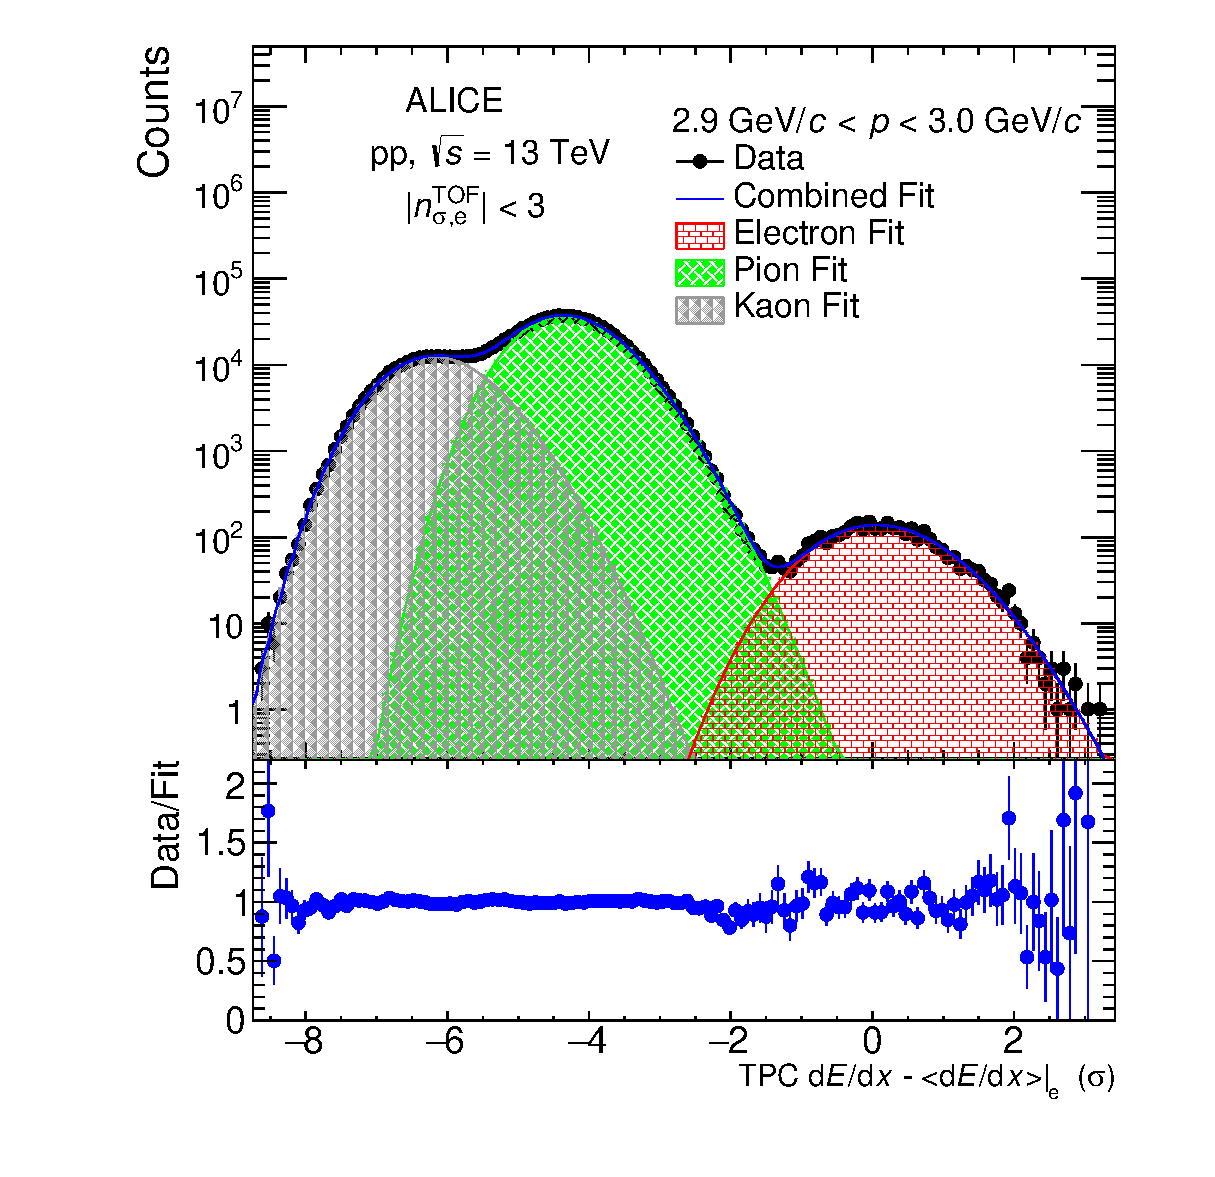
\includegraphics[scale = 0.35]{figures/Results/HFE_pp_LowB/TPCNsigma29to30_New.eps}
    \caption{TPC d$E$/d$x$ signal as a deviation from the expected electron energy loss after TOF selection (left) and Fit of $n^{\rm{TPC}}_{\sigma,\rm{e}}$ distributions of various species in pp collisions at $\sqrt{s}$ $=$ 13 TeV (right).} %{\color{blue} I see quite some issues here with the figure. we will for sure be asked why the kaon are not smooth in the right panel and why the fit at 0.2 GeV/c is not nice and what is the chi2 value we get. Don't we have better fit? Can the kaon be smoothened? Actually, do we need this figure at all (provocative ;))}}
    \label{fig:pp_13_TPCNsigma}
\end{figure}

 %In transverse momentum region 0.2 to 4 GeV/$c$, the particles are identified as electrons which satisfies the criteria of -1 $<$ $n^{TPC}_{\sigma,e}$ $<$ 3, which gives rise to the electron identification (eID) efficiency of 84$\%$. Moreover, the tracks with $|n^{TOF}_{\sigma,e}|$ $<$ 3, were accepted to overcome the ambiguities mentioned earlier. 
%The obtained electrons sample may still contain the contamination from the hadrons. The amount of this contamination is estimated by parameterizing the TPC d$E$/d$x$ distribution after TOF selection in different momentum regions for $p_{\rm T}$ $\leqslant$ 4 GeV/$c$, as done in previous analyses [ref]. 

In the analysis using TPC--EMCal detectors, for $p_{\rm T}$ $>$ 3 GeV/$c$, tracks with $-1 < n^{\rm{TPC}}_{\sigma,\rm{e}}$ $<$ 3 are selected. The electron sample was obtained by selecting candidates with $0.85 < E/p < 1.2$, as electrons are expected to be around unity, while hadrons have lower $E/p$ values. To further reduce the amount of hadron contamination, a condition on the shape of the electromagnetic shower ~\cite{Alessandro:2006yt}, $\sigma^{2}_{\rm{short}}$ and $\sigma_{\rm{long}}^{2}$, was
applied. $\sigma^{2}_{\rm{short}}$ and $\sigma_{\rm{long}}^{2}$ stands for the eigenvalues of the dispersion matrix of the shower shape ellipse defined by the energy distribution within the EMCal cluster ~\cite{Awes:1992yp, Acharya:2017hyu}. A \pt dependent selection of $0.02 < \sigma_{\rm{long}}^{2} < 0.9/0.7/0.5$ 
for $p_{\rm T} < 12 , 12- 20,  > 20$ GeV/$c$
in both pp collisions and in p-Pb collisions were chosen, as it reduces the hadron contamination while not significantly affecting the electron signal efficiency.  The lower threshold of $\sigma^{2}$ is chosen to remove contamination caused by neutrons hitting the readout electronics. The hadron contamination in the electron sample was estimated by measuring $E/p$ for hadrons with $n^{\rm{TPC}}_{\sigma,\rm{e}} < -3.5 $ for pp collisions  and $n^{\rm{TPC}}_{\sigma,\rm{e}} < -4$ for p-Pb collisions. The hadron $E/p$ distribution is scaled to match the electron candidate's $E/p$ distribution in the range $E/p<0.7$, as shown in Fig.~\ref{fig:pp_13_EbyP}. The electron yield was obtained by integrating the $E/p$ distribution for $0.85 < E/p < 1.2$. In pp (p-Pb) analysis, the hadron contamination was negligible at low $p_{\rm{T}}$, and increased to around $23\%$ ($25\%$) at $p_{\rm{T}} $ $=$ 35 (26) GeV/$c$, which was subtracted from the electron sample.

\begin{figure}[h!]
    \centering
    \includegraphics[height=6cm,width=7cm]{{figures/Results/HFE_ppNormalB/EbyP_MB}.pdf}
    \includegraphics[height=6cm,width=7cm]{{figures/Results/HFE_ppNormalB/EbyP_EG1}.pdf}
    \caption{E/p distribution for pp 13 TeV for MB (left) and EG1 (right) triggers}
    \label{fig:pp_13_EbyP}
\end{figure}

%\begin{table}[h]
%\caption{Summary of the particle identification criteria imposed on the inclusive electron candidates}
%\centering
%\begin{tabular}{c c c c c}
%\hline\hline
%Track and PID & pp 13 TeV  & pp 13 TeV & p--Pb 8 TeV & p--Pb 8 TeV\\ 
%cuts & $p_{\rm T}$ $\leqslant$ 4 GeV/$c$ & $p_{\rm T}$ $>$ 4 GeV/$c$ &  $p_{\rm T}$ $\leqslant$ 4 GeV/$c$ &  $p_{\rm T}$ $>$ 4 GeV/$c$\\ [0.5ex]
%\hline 
%TPC $\frac{dE}{dX}$ - $<$TPC$\frac{dE}{dX}>\mid _{el}$ & -1 to 3 $\sigma$  & -1 to 3 $\sigma$ &  0 to 3 $\sigma$ &  0 to 3 $\sigma$\\
%  &  &  &  &\\
%TOF $t$ - $<$TOF$t>\mid _{el}$ & -3 to 3 $\sigma$ & -- & -3 to 3 $\sigma$ & --\\
 %&  &  & &\\
%EMCal & -- &  & -- &  \\
% &  &  & &\\
%\hline
%\end{tabular}
%\label{Table:InclusivePIDSelection}
%\end{table}



\subsection{Subtraction of electrons from non heavy-flavour sources}
The selected inclusive electron sample contains electrons from open heavy-flavour hadron decays and from  different sources of background:

\begin{itemize}
    \item electrons coming from Dalitz decay of light-neutral mesons such as $\pi^{0}$, $\eta$ as well as conversion of photons in the detector material, termed as photonic electrons in the text. 
    \item di-electrons from J/$\psi$ (J/$\psi$ $\rightarrow$ $e^{+}e^{-}$) and low-mass vector mesons ($\rho$ $\rightarrow$ $e^{+}e^{-}$, $\omega$ $\rightarrow$ $e^{+}e^{-}$, $\phi$ $\rightarrow$ $e^{+}e^{-}$).
\item electrons from weak decays $\rm K^{0/\pm}$ $\rightarrow$ $e^{\pm}$ $\rm \pi^{0/\mp}$ $\rm \nu_{e}$ (Ke3). 

\item electrons from W and Z decays, and from prompt photons.
\end{itemize}

In pp collisions, the ratio of signal over background electrons is about 0.08 at \pt $=$ 0.2 GeV/$c$ which is very small and it increases upto 12.3 at \pt $=$ 35 GeV/$c$. In \pPb collisions, the ratio of signal over background electrons is about 2.65 at \pt $=$ 0.5 GeV/$c$ and it increases upto 8.39  at \pt $=$ 26 GeV/$c$.  The dominant source of background electrons are photon conversion in the detector material and Dalitz decays of light-neutral mesons. These contributions are removed using an invariant mass technique~\cite{Adam:2015qda}, where electron-positron pairs are defined by pairing the selected electrons with opposite-charge electron partners to form unlike-signed pairs (ULS) and calculating their invariant mass ($ m_{\rm e^{+}e^{-}}$). Partner electrons are selected applying similar but looser track quality and particle identification criteria than those used for selecting signal electrons to increase the efficiency of finding the partner, as summarized in Table~\ref{Table:AssocatedTrackSelection}. The electron-positron pairs from photonic background have a small invariant mass, while heavy-flavour decay electrons can form
ULS pairs mainly through random combinations with other electrons.
%, resulting in a continuous invariant mass distribution. 
The combinatorial contribution is estimated from the invariant mass distribution of
like-signed electron (LS) pairs. The photonic background contribution is then evaluated by subtracting the LS distribution from the ULS distribution in the invariant mass region $m_{\rm e^{+}e^{-}} < 0.14$ GeV/$c$. The efficiency of finding the partner electron, called as tagging efficiency ($\epsilon_{tag}$) from hereon, is estimated using the Monte-Carlo (MC) simulations. In pp and p-Pb analysis, the MC sample is obtained using PYTHIA 6~\cite{Sjostrand:2006za} and HIJING~\cite{Wang:1991hta} generator respectively.  The generated particles are propagated through the ALICE apparatus using GEANT3~\cite{Brun:1073159}.
In pp analysis, the tagging efficiency in the low B and nominal B data samples is $\sim 45\%$ at 0.5 \GeVc, increasing to $\sim 80\%$ at $\pt > 5 \GeVc$. 
%In the nominal B dataset, the tagging efficiency was $\sim 45\%$ at 0.5 \GeVc, increasing to $\sim 85\%$ for .
%{\color{cyan} In pp analysis, the tagging efficiency was around 55--65\% (45--55\%) with low B (nominal B) at low $p_{\rm{T}}$ ($p_{\rm{T}} < 1.0$ GeV/$c$) analysis increasing to around 85\% at high $p_{\rm{T}}$ bins ({\color{purple}$p_{\rm{T}} > 15$ }GeV/$c$). {\color{purple} $=>$ In pp analysis, the tagging efficiency was around 55--65\% for low B at low $p_{\rm{T}}$ ($p_{\rm{T}} < 1.0$ GeV/$c$). For  nominal B , the tagging efficiency was found to be around 45--65\% for low $p_{\rm{T}}$ ($p_{\rm{T}} < 3.0$ GeV/$c$)  analysis increasing to around 85\% at high $p_{\rm{T}}$ bins ({\color{purple}$p_{\rm{T}} > 15$ }GeV/$c$)}. 
In p-Pb analysis, the tagging efficiency is around {40--70\%}  at low $p_{\rm{T}}$ ($p_{\rm{T}} < 3$ GeV/$c$) increasing to around 80\% at high $p_{\rm{T}}$ ($p_{\rm{T}} > 3$ GeV/$c$).

\begin{table}[h]
\caption{Summary of the track selection criteria imposed on the associated electron candidates for different datasets and electron identification strategies.}

\centering
\small
\begin{tabular}{c |c c c | c c}
\hline\hline
%Track and PID & \multicolumn{3}{c|}{ pp 13 TeV}  & \multicolumn{2}{c|}{p--Pb 8 TeV} \\ 
%cuts & $p_{\rm T}$ $<$ 0.5 GeV/$c$  & 0.5 $ \leqslant p_{\rm T} < $ 3 GeV/$c$ & $p_{\rm T}$ $>$ 3 GeV/$c$ &  $p_{\rm T}$ $\leqslant$ 3 GeV/$c$ &  $p_{\rm T}$ $>$ 3 GeV/$c$\\ [0.5ex]

 & \multicolumn{3}{c|}{pp 13 TeV} & \multicolumn{2}{c}{p--Pb 8.16 TeV}  \\ 
 Track and PID  & Low B & Nominal B  & Nominal B & Nominal B & Nominal B \\
  cuts & TPC--TOF & TPC--TOF  & TPC--EMCal & TPC--TOF & TPC--EMCal \\
\hline 
$p_{T}^{min}$ & 0.0 GeV/c   &{ 0.1 GeV/c}&   { 0.1 GeV/c}& 0.1 GeV/c &  0.1 GeV/c\\
$|\eta|$ & $<$ 0.8  &  { $<$ 0.9 } &  { $<$0.9 } & $<$ 0.8 & $<$ 0.8 \\
No. of TPC & $\geq$ 60  &$\geq$ 60 & $\geq$ 60 & $\geq$ 60 & $\geq$ 60\\
d$E$/d$X$ clusters (PID) & & &  & &\\
Number of ITS hits & $\geq$ 2 & $\geq$ 2& $\geq$ 2 & $\geq$ 2& $\geq$ 2\\

%\item Ratio found / findable TPC clusters $>$ 0.6
$\chi^{2}$ /clusters of & $<$ 4 &$<$ 4 & $<$ 4 &$<$ 4&$<$ 4\\
momentum fit in TPC &  &  &&\\
%Ratio found / findable TPC clusters & $>$ 0.6 & $>$ 0.6 \\
% (\textcolor{red}{2})
$|\rm DCA_{xy}|$ & $<$ 1 cm &$<$ 1 cm  & $<$ 1 cm & $<$ 1 cm& $<$ 1 cm\\
$|\rm DCA_{z}|$ & $<$ 2 cm & $<$ 2 cm & $<$ 2 cm & $<$ 2 cm & $<$ 2 cm\\
%Kink mothers and daughters & excluded & excluded \\
%TOF $t$ - $<$ TOF $t>\mid _{el}$ in between & -3 to 3 $\sigma$ & -3 to 3 $\sigma$ & not used\\
%TPC $\frac{dE}{dX}$ - $<$ TPC $\frac{dE}{dX}>\mid _{el}$ in between  & -1 to 3 $\sigma$  & -1 to 3 $\sigma$ &  -3 to 3 $\sigma$\\

\hline
\end{tabular}
\label{Table:AssocatedTrackSelection}
\end{table}

Due to the requirement of hits in the pixel layers, the contribution of electrons from Ke3 was found to be negligible for $p_{\rm{T}} > 0.5$ GeV$/c$. At lower $p_{\rm{T}}$, the relative contribution of electrons from Ke3 becomes non-negligible and is hence subtracted from the fully corrected cross section. The Ke3 contribution was estimated using a parameterization of the ratio of Ke3 to photonic electrons obtained from previous analyses using the so-called cocktail approach~\cite{Acharya:2018upq,Abelev:2014gla,Abelev:2012xe}. The parameterization was found to be independent of collision energies and hence used here in the analysis of pp collisions at 13 TeV. 

Other background contribution of  di-electrons from J/$\psi$ and low-mass vector mesons are negligible~\cite{Acharya:2018upq} compared to the contribution from photonic electrons and is therefore not subtracted. Electrons from W and Z decays form significant background at high $p_{\rm{T}}$ ($>20$ GeV/$c$), obtained using the POWHEG event generator~\cite{Oleari:2010nx} is subtracted from the fully corrected cross section. The contribution increases from 1\% (1\% ) at $p_{\rm{T}} = 15$ GeV/$c$ to
about {3\%} (3 \% ) at $p_{\rm{T}} = 20$ GeV/$c$ and 25\% at $p_{\rm{T}} = 35$ GeV/$c$ w.r.t heavy-flavour decay electron yield in pp  (p-Pb) collisions.


%These contributions are removed using the invariant mass method~\cite{Adam:2015qda}. The photonic electrons are produced as unlike-sign electron-positron pairs (ULS) with small invariant mass ($m_{e^{+}e^{-}}$). The combinatorial background in the invariant mass distribution is obtained by calculating the invariant mass of like-sign (LS) electron pairs. The photonic electron contribution is obtained by subtracting the LS paired  

%Subtraction of the dominant background component to the signal electrons was performed using photonic-electron tagging method. Photonic background dominates the inclusive electron spectrum below $p_{\rm T}$ $=$ 1.5 GeV/$c$ while its contribution becomes smaller at high $p_{\rm T}$. The photonic electrons come from the pairs of electron-positron originating from either photon conversions or dalitz decay of light mesons with small invariant mass ($m_{e^{+}e^{-}}$). 
%Contribution from these electrons is obtained by tagging electron (positron) track with the track identified as positron (electron) in the same event, whereas, the combinatorial background is built by obtaining the invariant mass distribution of like-sign pairs within same pair invariant mass interval in both cases.


%The limited detector acceptance and decay kinematics prevent reconstruction of all photonic electrons. So the raw yield of these electrons should be corrected for the efficiency which takes these limitations into account, called tagging efficiency ($\epsilon_{tag}$) from hereon. This efficiency is estimated using the Monte Carlo (MC) simulations. 
%In p--Pb collisions, the sample of events was generated using HIJING generator while PYTHIA6 was used in case of pp collisions. 

%In case of $p_{\rm T}$ $>$ 4 GeV/$c$, one $c\bar{c}$ or $b\bar{b}$ pair decaying semileptonically was embedded in each event due to lack of statistics at higher transverse momentum. This is followed by transport of these particle with the help of GEANT3 and their detailed reconstruction. 


\subsection{EMCal trigger rejection factor}
The electron yield obtained using the EMCal triggered
data sample is enhanced at high $p_{\rm T}$, and is corrected by the trigger rejection factor (RF). The RF quantifies the fraction of MB interaction triggers which are rejected by the  EMCal trigger condition. It was
obtained via a data-driven method using the ratio of the cluster energy distribution in triggered-data to the one in minimum-bias triggered data, which gives the turn-on curve. The turn-on curve is determined in multiplicity integrated and in different multiplicity intervals in pp and \pPb collisions. Figure~\ref{fig:RF} shows an example of the turn-on curve for multiplicity integrated pp and \pPb collisions for both trigger energy thresholds (EG1 and EG2).

\begin{figure}[h!]
    \centering
    \includegraphics[width=0.48\linewidth]{{figures/Results/HFE_ppNormalB/RF_trackmatchCluster}.pdf}
    \includegraphics[width=0.48\linewidth]{figures/Results/HFE_pPb/RF_extendedpT_extendedFit.pdf}
    
    \caption{Trigger Rejection Factor for EG2 and EG1 triggers in pp collisions at $\sqrt{s}=13$ TeV (left) and in \pPb collisions at $\sqrtsNN = 8.16$ TeV (right).}
   \label{fig:RF}
\end{figure}


The rejection factor was obtained by fitting a Fermi function~\cite{Fermi:1934hr, Wilson:1968pwx} to the turn-on curve from around the trigger threshold up to higher $p_{\rm T}$ where the distribution flattens. The values obtained for the rejection factor are summarised in Table~\ref{table:RF}. The uncertainties on the values of the rejection factor were obtained using different fit ranges on the plateau.

\begin{table}[h!]
\caption{Multiplicity integrated values of the EMCal trigger rejection factor with their uncertainties for the EG2 and EG1 triggered datasets in pp and \pPb collisions.}
    \centering
    \begin{tabular}{c| c c | c c}
    \toprule
    \multicolumn{1}{c|}{}&
    \multicolumn{2}{c|}{pp $\sqrt{s} = 13 \TeV$}& \multicolumn{2}{c}{\pPb $\sqrt{s_{\rm NN}} = 8.16 \TeV$}\\
%   \midrule
   %    &  &  pp &  & p--Pb\\
                Trigger   & EG2 & EG1 & EG2 & EG1 \\
                \midrule
     RF value & { 406 $\pm$ 12 } & { 5040 $\pm$ 202 } &  255.65 $\pm$ 1.50 & 815.76 $\pm$ 8.43 \\
     \bottomrule
    \end{tabular}
    \label{table:RF}
\end{table}


\subsection{Efficiency correction and normalization}\label{section:corrections}
The raw number of electrons from heavy-flavour hadron decays obtained after the subtraction of hadron contamination, photonic and other background contribution, is divided by the number of events analysed (${N_{\rm events}}$), 
%by the value of $p_{\rm T}$ at the centre of each bin and 
 width of the $\pt$ range ($\Delta p_{\rm T}$), by the width $\Delta y$ of the covered rapidity interval, by the geometrical acceptance ($\epsilon^{\rm geo}$) times the track reconstruction ($\epsilon^{\rm reco}$) and electron identification efficiencies ($\epsilon^{\rm eID}$) and a factor of two to obtain the charge averaged invariant differential yield which is further multiplied by minimum bias trigger cross section to get the $p_{\rm T}$-differential production cross section of electrons. The MB trigger cross section for pp collisions at $\sqrt{s}$ $= 13$ TeV and for \pPb collisions at $\sqrt{s_{\rm{NN}}}$ $=8.16$ TeV was $\sigma_{\rm MB}$ $=$ 57.8 $\pm$ 2.9 mb and 2100 $\pm$ 60 mb respectively.  
 %{\color{blue} (is this value same for both lowB and normal B?) {(\color{cyan} Yes, at the moment it is taken to be same)} and {\color{teal} 2100 $\pm$ 60 mb}} respectively.  

\begin{equation}
 \frac{d^2\sigma}{dp_{\rm T}dy} = \frac{1}{2}  \frac{1}{\Delta y \Delta p_{\rm T}} \frac{{N_{\rm{raw}}}} {\epsilon^{\rm{geo}} \times \epsilon^{\rm reco} \times  \epsilon^{\rm {eID}} } \frac{\sigma_{\rm{MB}}}{N_{\rm {events}}}
%\frac{1}{2 \pi p_{\rm{T}}} \frac{d\sigma}{dp_{\rm T}dy} = \frac{1}{2} \frac{1}{2 \pi {p_{\rm T}^{\rm centre}}}  \frac{1}{\Delta y \Delta p_{\rm T}} \frac{{N_{\rm{raw}}}} {\epsilon^{\rm{geo}} \times \epsilon^{\rm reco} \times  \epsilon^{\rm {eID}} } \frac{\sigma_{\rm{MB}}}{N_{\rm {events}}} 
\end{equation}

The above mentioned acceptance and track reconstruction efficiencies were computed using MC simulations. In pp and \pPb analyses, the MC sample was obtained using PYTHIA 6~\cite{Sjostrand:2006za} and HIJING~\cite{Wang:1991hta} event generators respectively, with the generated particles propagated through the ALICE apparatus using GEANT 3~\cite{Brun:1073159}.  To increase the sample of electrons from charm- and beauty-hadron decays, a sample of charm and beauty quarks generated with PYTHIA 6 is embedded into each MC event. The electron identification (eID) efficiency for TOF, TPC and the EMCal detectors were obtained separately, and then multiplied according to the detectors used in the analysis to compute the full eID efficiency $\epsilon^{\rm eID}$. The eID efficiency of TOF detector was obtained using the above mentioned MC sample and was found to be 60--70$\%$ (40--65$\%$) for  0.5 $<$ $p_{\rm T}$ $<$ 1.5 GeV/c increasing upto 75$\%$ (70$\%$) at 4 GeV/c in low (nominal) B analysis. The TPC eID efficiency was determined using a data-driven approach based on the $n^{\rm{TPC}}_{\sigma,\rm{e}}$ distribution~\cite{Abelev:2012xe}, and was found to be $\sim 88\%$ at $p_{\rm T}= 0.2$ GeV/$c$, increasing to $\sim 89\%$ at $p_{\rm T} > 0.5$ GeV/$c$ for $-1 < n^{\rm{TPC}}_{\sigma,\rm{e}}< 3$ range, for low B data sample. In nominal B dataset, it is found to be $\sim 86\%$ at $p_{\rm T}= 0.5$ GeV/$c$ and $\sim 88\%$ at $p_{\rm T} > 4$ GeV/$c$ for $-1 < n^{\rm{TPC}}_{\sigma,\rm{e}}< 3$ range. In \pPb dataset, similar TPC eID efficiency is observed. It is found to be be $\sim 86\%$ at $p_{\rm T}= 0.5$ GeV/$c$ and $\sim 89\%$ at $p_{\rm T} > 4$ GeV/$c$ for $-1 < n^{\rm{TPC}}_{\sigma,\rm{e}}< 3$ range.  The eID efficiency with EMCal, employing the $E/p$  and shower shape cut was estimated using Monte-Carlo simulations. It was found to be $\sim$ 60\% at 3 GeV/$c$ increasing upto $\sim$ 80 \% at 10 GeV/$c$ and at higher \pt for pp collisions. 
%The product of the overall acceptance and efficiency ($\epsilon^{\rm geo} \times \epsilon^{\rm reco} \times \epsilon^{\rm eID}$) as function of $p_{\rm{T}}$ for the TPC-TOF analysis and for the TPC-EMCal analysis are shown in Figure~\ref{Fig:TotEffi} for both pp and \pPb collisions.
The total reconstruction efficiency ($\epsilon^{\rm{geo}} \times \epsilon^{\rm reco} \times  \epsilon^{\rm {eID}}$) for different data sets and with different detectors are presented in Figure~\ref{Fig:ppHFEEff}. Due to better track matching between TPC and TOF detectors with low magnetic field, a higher reconstruction efficiency was observed in low B data sample compared to the nominal B field sample.

\begin{figure}[!ht]


 \begin{center}
      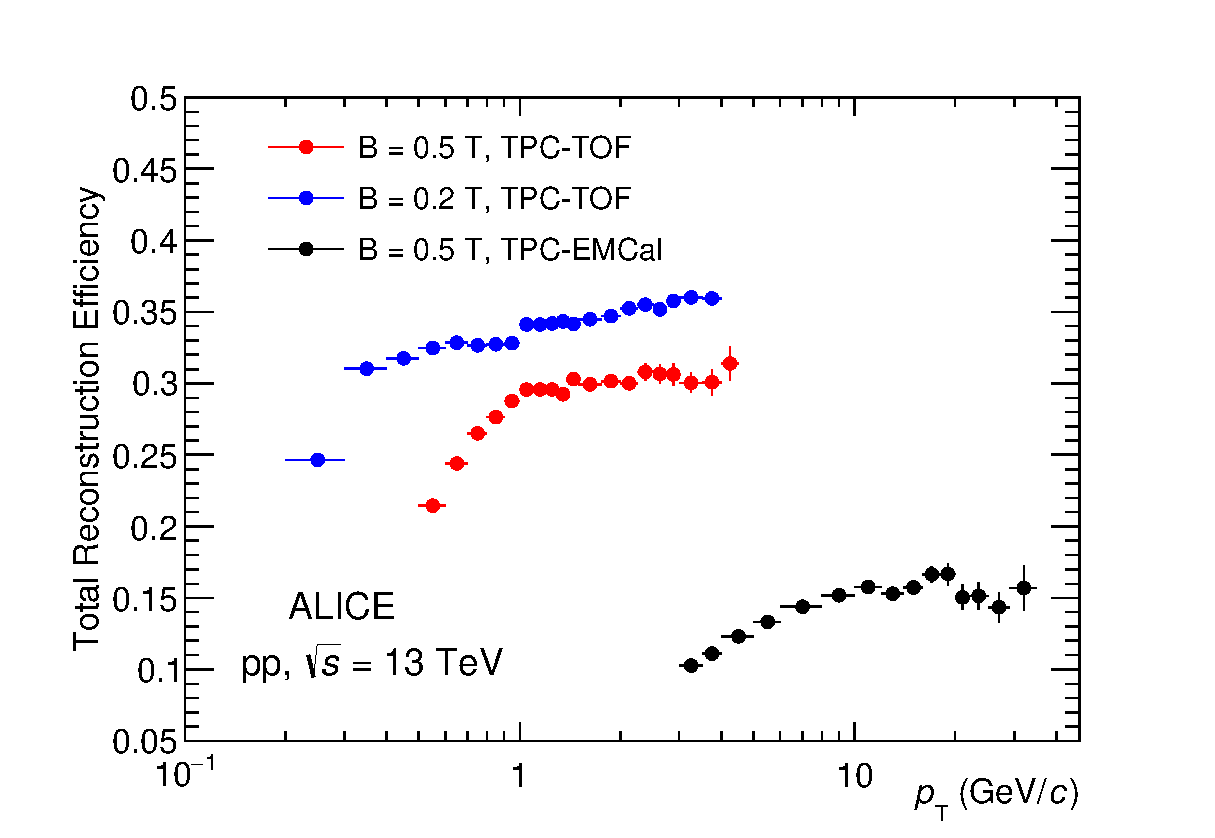
\includegraphics[width=0.48\linewidth]{figures/Results/HFE_pp_LowB/CompWithNormalB_LowB_logx.eps}
      \includegraphics[width=0.46\linewidth]{figures/Results/HFE_pPb/TotalReconstructionEfficiency.pdf}
      \end{center}

\caption{Total reconstruction efficiency of electrons from heavy-flavour hadron decays in pp collisions at $\sqrt{s}$ $=$ 13 TeV with normal and low magnetic field using TPC-TOF and TPC-EMCal (left) and in \pPb collisions $\sqrtsNN=8.16$ TeV using TPC-TOF and TPC-EMCal (right).}        
\label{Fig:ppHFEEff}
\end{figure}


%Dedicated MC simulations are used to determine the efficiencies. For pp analysis, each event is embedded with one $c\bar{c}$ or $b\bar{b}$ pair decaying semileptonically in heavy-flavour enriched PYTHIA MC sample. HIJING event generator is used for p--Pb analysis in which heavy-flavour signal is added using PYTHIA.
\section{Systematics uncertainty studies}\label{sec:systematics}
The systematic uncertainties on the measurements of invariant yield in pp and \pPb collisions were performed separately for TPC--TOF and TPC--EMCal analyses as a function of $p_{\rm{T}}$. The uncertainties on the invariant yield at low $p_{\rm{T}}$ obtained using the low B datatset were also performed independently. For the self-normalised yield measurements in pp and \pPb collisions, the systematic uncertainties were estimated directly on the self-normalised yield for each multiplicity class and $p_{\rm{T}}$ intervals. The different sources of systematic uncertainties are further discussed in this section and the assigned values are summarized in Tables~\ref{tab:SystematicSummaryTPCTOC}, ~\ref{tab:SystematicSummaryTPCEMCal} and ~\ref{tab:summarysystSN}

The systematic uncertainty on the track selection were obtained by multiple variations of the selection criteria.  The minimum number of space points in the TPC and the hits in the ITS were varied to estimate the uncertainty. For low B sample in pp collisions, the uncertainty for the track matching between the ITS and TPC was 2$\%$ at $\pt \sim 0.2 \GeVc$ increasing upto $4.0\%$ at 4 \GeVc, whereas, the uncertainty for the track matching between the TPC and TOF detector was $4\%$ at $\pt \sim 0.2 \GeVc$ and $2\%$ at 4 \GeVc. In case of the nominal B dataset, uncertainty for the TPC--TOF track matching is  $\sim$2$\%$  and the ITS--TPC track matching is $\sim$3$\%$ in whole $\pt$ range. In the pPb analysis uncertainty for the TPC--TOF track matching is also observed to be  $\sim$2$\%$ in whole $\pt$ range.

%{\color{cyan}2$\%$ for 0.2 $\leq$ $p_{\rm T}$ $\leq$ 1.0, 3$\%$ for 1.0 $\leq$ $p_{\rm T}$ $\leq$ 2.0 and 4.0$\%$ 2.0 $\leq$ $p_{\rm T}$ $\leq$ 4.0 GeV/c, and TPC and TOF as 4$\%$ for 0.2 $\leq$ $p_{\rm T}$ $\leq$ 0.3 and 2.0$\%$ 0.3 $\leq$ $p_{\rm T}$ $\leq$ 4.0 GeV/c.}

The uncertainty on the reconstructed electron sample can originate from  potential biases in the procedure employed to select electron candidates and estimate the hadron contamination, and an uncertainty related to the electron reconstruction efficiency arising from imprecision in the description of the detector response in the MC. It was studied by varying the electron identification selection criteria using $n^{\rm{TPC}}_{\sigma,\rm{e}}$ in the TPC and $E/p$ and $\sigma^2_{\rm{long}}$ in the EMCal. Further the uncertainty on the estimation and removal of hadron contamination in the TPC--TOF analysis was obtained by varying the analytical function to parameterize the TPC ${\rm{d}}E/{{\rm{d}}x}$, which had negligible effect at low $p_{\rm{T}}$ upto 3.0 GeV/c. For the TPC--EMCal analysis, the scaling region of the hadron $E/p$ was varied between 0.2 and 0.7, found to be negligible at low $p_{\rm{T}}$ upto 20 GeV/$c$ with a maximum value of $5\%$ at 35 GeV/$c$.

The uncertainty on the subtraction of photonic electrons is related to the efficiency of finding partner electron and was studied by varying the selection for partner tracks, with the number of space points in the TPC cluster and minimum $p_{\rm{T}}$, and the invariant mass cut of di-electron pairs. The subtraction of Ke3 electrons decays in pp collisions for $p_{\rm{T}} < 0.5$ GeV$/c$ is affected by the uncertainty on the parameterization of the ratio of Ke3 to photonic electrons and was found to result in an uncertainty of 15\% at $p_{\rm{T}} = 0.2~\GeVc$ and negligible at $p_{\rm{T}}=0.5$ GeV$/c$. 

The uncertainty on the contribution of electrons from W and Z decays was obtained by varying the parton distribution function from { CT10nlo\cite{Guzzi:2011sv} to CTEQ6l\cite{Pumplin:2002vw}} in the POWHEG event generator, and the resulting variation in the yield of electrons from heavy-flavour decays was found to be negligible. 

The systematic uncertainty on trigger rejection factor was obtained by varying the fitting region of the trigger turn-on curve and also fitting it with a linear function in the plateau region. A systematic uncertainty of 3\% (3\%) in EG2 trigger and 8\% (4\%) in EG1 trigger was assigned in \pPb (pp) collisions.

The systematic uncertainity on the measurement of the self-normalised yield in pp and \pPb collisions from all  the sources mentioned above were independently estimated and is summarized in Table~\ref{tab:summarysystSN}. As the geometrical acceptances, reconstruction efficiencies are independent of \dnchdeta in the measured multiplicity range, these corrections and their corresponding systematic uncertainties largely cancel in the ratio $\dndeta/\left<\dndeta\right>$, thus resulting in a lower systematics for self-normalised yield compared to the one for $p_{\rm{T}}$ spectra. 

% TPC--TOF(B=0.2T) && TPC--TOF(B=0.5T) && TPC-EMC
% 0.2-X && x-4 && 4-6 (MB) && 6-12 (EG2) && 12-36 (EG1)
% && x-y\% && x-y\% && x-y\% && x-y\%
The total systematic uncertainties on the $p_{\rm{T}}$ spectra and self-normalised yield were calculated by summing the different contributions in quadrature, as they are considered to be uncorrelated. 
  

\begin{table}[th!]
 \centering
 \caption{Sources of systematic uncertainties and its assigned values in pp collisions at 13 TeV for B = 0.2 T (0.2 $<p_{\rm T}$ (GeV/$c$) $<$ 0.5) and B = 0.5 T data sets with TPC--TOF (0.5 $<p_{\rm T}$ (GeV/$c$) $<$ 4) and TPC--EMCal (4 $<p_{\rm T}$ (GeV/$c$) $<$ 35) detectors. The values presented as a range corresponds to the the lowest and highest \pt bin. } %for low and normal magnetic field configuration.}
  \resizebox{\textwidth}{!}{  
\begin{tabular*}{\textwidth}{@{\extracolsep{\fill}}  l| ccc}
    \toprule
    {Observable} & { 0.2 $<p_{\rm T}$ (GeV/$c$) $<$ 0.5} & { 0.5 $<p_{\rm T}$ (GeV/$c$) $<$ 4} & { 4 $<p_{\rm T}$ (GeV/$c$) $<$ 35}\\
        {} & {(low B, TPC--TOF)} & { (nominal B, TPC--TOF)} & { (nominal B, TPC-EMal)}\\

\midrule
\midrule
{ Track selection } & {Negligible} & 1$\%$ & 3$\%$ \\
\midrule
{Electron Identification} & {5$\%$} &  {5$\%$ - Negligible}& 6\%- 12\% \\\midrule
%\multirow{2}*{Photonic Electron} & {} &  & \\
{Photonic Electron} & {20$\%$ -- 11$\%$} & 7\% - 1\%  &  Negligible\\
{Selection} & {} &   &  \\\midrule  
{Hadron contamination } & {Negligible} & Negligible - 2\%  &  Negligible -7\% \\\midrule  
{ TPC--TOF matching} & { 4$\%$ -- 2$\%$} & 2\% & \\\midrule  
{W/Z $\rightarrow$ e } & {-} &- &  Negligile\\ \midrule
 {SPD hit requirement } & {25$\%$ -- 15$\%$} &  10\% - 3\% & { 5\% - Negligible }\\\midrule
{Rejection Factor } & { -} & - & 3\%-4\% \\ \midrule
{ITS--TPC matching } & { 2\%} & 3\%  &  3\%\\ \midrule
{$\pi^{0}$, $\eta$ weights } & { 3\% -- 1$\%$} & - &  -\\
\midrule
{Ke3 subtraction } & {15\% -- 1$\%$} & - & - \\
\midrule
  \end{tabular*}
  }
   \label{tab:SystematicSummaryTPCTOC}
\end{table}

% \begin{table}[H]
%  \centering
%  \caption{Sources of systematic uncertainties and its assigned values in pp collisions at 13 TeV for B = 0.2 T and B = 0.5 T data sets.} %for low and normal magnetic field configuration.}
%  \label{tab:SystematicSummaryTPCTOC}
%   \resizebox{\textwidth}{!}{  
%     \begin{tabular*}{\textwidth}{@{\extracolsep{\fill}}  cc| cc|c|cc}
%     \toprule
%      \multicolumn{2}{l}{}
%   & \multicolumn{2}{c}{Observable} &  \multicolumn{1}{c}{TPC--TOF(Low B)}&   \multicolumn{2}{c}{Normal B} \\
% \midrule
%   \multicolumn{2}{c}{\pt (\GeVc)}&\multicolumn{2}{c}{}
%   & \multicolumn{1}{c}{0.2$-$4}& \multicolumn{1}{c}{0.5$-$4}& \multicolumn{1}{c}{4$-$30}\\
  
%   \midrule
%      \multicolumn{2}{l|}{}
%   & \multicolumn{2}{l|}{TPC Clusters ($\#$ crossed rows)} & \multicolumn{1}{c}{}& \multicolumn{1}{c}{}& \multicolumn{1}{c}{} \\
 
%       \multicolumn{2}{c|}{ Track  cuts}
%   & \multicolumn{2}{c|}{TPC Clusters for PID}  & \multicolumn{1}{c}{Negligible}& \multicolumn{1}{c}{}& \multicolumn{1}{c}{3.0$\%$}\\
%     \multicolumn{2}{c|}{}
%     & \multicolumn{2}{c|}{DCA$_{xy}$(cm),DCA$_{z}$(cm)}   & \multicolumn{1}{c}{}& \multicolumn{1}{c}{}& \multicolumn{1}{c}{} \\
   
   
%  \midrule  
%      \multicolumn{2}{c|}{}
%      & \multicolumn{2}{c|}{}  & \multicolumn{1}{c}{}& \multicolumn{1}{c}{5.0$\%$}& \multicolumn{1}{c}{6 (4--16 GeV/c)} \\
%       \multicolumn{2}{c|}{PID cuts for}
%      & \multicolumn{2}{c|}{$n{\rm ^{TPC}_{\sigma,e}}$ selection}  & \multicolumn{1}{c}{5$\%$(0.2 -- 2.0 GeV/c}& \multicolumn{1}{c}{(0.5 -- 1.0}& \multicolumn{1}{c}{12 (16--35 GeV/c)} \\
     
       
%   \multicolumn{2}{c|}{ electron}   & \multicolumn{2}{c|}{$n{\rm ^{TOF}_{\sigma,e}}$ selection} &  \multicolumn{1}{c}{}& \multicolumn{1}{c}{ GeV/c)}& \multicolumn{1}{c}{} \\
   
%     \multicolumn{2}{c|}{identification}
%      & \multicolumn{2}{c|}{E/p}  & \multicolumn{1}{c}{}& \multicolumn{1}{c}{}& \multicolumn{1}{c}{} \\
%       \multicolumn{2}{c|}{}
%      & \multicolumn{2}{c|}{Shower Shape}  & \multicolumn{1}{c}{}& \multicolumn{1}{c}{}& \multicolumn{1}{c}{} \\
   
%   \midrule
   
   
%     \multicolumn{2}{c|}{Photonic} 
%  & \multicolumn{2}{c|}{Min. \pt (\GeVc) } &  \multicolumn{1}{c}{ 20$\%$ (0.2 -- 0.3 GeV/c)}& \multicolumn{1}{c}{-}& \multicolumn{1}{c}{-}\\
%       \multicolumn{2}{c|}{background}
%   & \multicolumn{2}{c|}{Associated TPC clusters}  & \multicolumn{1}{c}{15$\%$ (0.3 -- 0.4 GeV/c)}& \multicolumn{1}{c}{-}& \multicolumn{1}{c}{-} \\
%     \multicolumn{2}{c|}{ selection}
%     & \multicolumn{2}{c|}{Invariant mass (\rm{GeV}/$c^2$)}  & \multicolumn{1}{c}{11$\%$ (0.4 -- 0.5 GeV/c)}& \multicolumn{1}{c}{-}& \multicolumn{1}{c}{-} \\
%      &   & \multicolumn{2}{c|}{}  & \multicolumn{1}{c}{ 7.0$\%$ (0.5 -- 0.9 GeV/c)}& \multicolumn{1}{c}{}& \multicolumn{1}{c}{-} \\
%       &   & \multicolumn{2}{c|}{}  & \multicolumn{1}{c}{ 3.0$\%$ (0.9 -- 1.3 GeV/c)}& \multicolumn{1}{c}{}& \multicolumn{1}{c}{-} \\
%     \midrule
%       \multicolumn{2}{c|}{ } 
%  & \multicolumn{2}{c|}{Hadron contamination} &  \multicolumn{1}{c}{ 2.0$\%$ (3.0 -- 4.0 GeV/c)}& \multicolumn{1}{c}{7(29-35)}& \multicolumn{1}{c}{7(29-35)} \\
%   &   & \multicolumn{2}{c|}{}  & \multicolumn{1}{c}{-}& \multicolumn{1}{c}{}& \multicolumn{1}{c}{-} \\
%       \multicolumn{2}{c|}{Other}
%   & \multicolumn{2}{c|}{TPC--TOF matching}  & \multicolumn{1}{c}{ 4.0$\%$ (0.2 -- 0.3 GeV/c)}& \multicolumn{1}{c}{}& \multicolumn{1}{c}{} \\
%     &   & \multicolumn{2}{c|}{}  & \multicolumn{1}{c}{ 2.0$\%$ (0.3 -- 4.0 GeV/c)}& \multicolumn{1}{c}{}& \multicolumn{1}{c}{-} \\
%      \multicolumn{2}{c|}{}
%   & \multicolumn{2}{c|}{W/Z $\rightarrow$ e}  & \multicolumn{1}{c}{-}& \multicolumn{1}{c}{}& \multicolumn{1}{c}{-} \\
%  &   & \multicolumn{2}{c|}{}  & \multicolumn{1}{c}{-}& \multicolumn{1}{c}{}& \multicolumn{1}{c}{-} \\
%     \multicolumn{2}{l|}{}
%     & \multicolumn{2}{c|}{SPD hit requirement} & \multicolumn{1}{c}{ 25$\%$ (0.2 -- 0.3 GeV/c)}& \multicolumn{1}{c}{10($<$1.5),3($>$1.5)}& \multicolumn{1}{c}{5($<16$)} \\
%      &   & \multicolumn{2}{c|}{}  & \multicolumn{1}{c}{ 15$\%$ (0.3 -- 0.5 GeV/c)}& \multicolumn{1}{c}{}& \multicolumn{1}{c}{-} \\
%       &   & \multicolumn{2}{c|}{}  & \multicolumn{1}{c}{ 5$\%$ (0.5 -- 2.5 GeV/c)}& \multicolumn{1}{c}{}& \multicolumn{1}{c}{-} \\
%         \multicolumn{2}{l|}{}
%     & \multicolumn{2}{c|}{ $\left|\eta\right|$ }  & \multicolumn{1}{c}{Negligible}& \multicolumn{1}{c}{-}& \multicolumn{1}{c}{-} \\
%      &   & \multicolumn{2}{c|}{}  & \multicolumn{1}{c}{}& \multicolumn{1}{c}{}& \multicolumn{1}{c}{-} \\
%         \multicolumn{2}{l|}{}
%     & \multicolumn{2}{c|}{ Rejection Factor}  & \multicolumn{1}{c}{-}& \multicolumn{1}{c}{}& \multicolumn{1}{c}{2(Re-check)} \\
%   &  & \multicolumn{2}{c|}{ITS--TPC matching}  & \multicolumn{1}{c}{ 2.0$\%$ (0.2 -- 1.0 GeV/c)}& \multicolumn{1}{c}{}& \multicolumn{1}{c}{} \\
%     &  & \multicolumn{2}{c|}{}  & \multicolumn{1}{c}{ 3.0$\%$ (1.0 -- 2.0 GeV/c)}& \multicolumn{1}{c}{}& \multicolumn{1}{c}{} \\
%      &  & \multicolumn{2}{c|}{}  & \multicolumn{1}{c}{ 4.0$\%$ (2.0 -- 4.0 GeV/c)}& \multicolumn{1}{c}{}& \multicolumn{1}{c}{} \\
%     &  & \multicolumn{2}{c|}{$\pi^{0}$, $\eta$ weights}  & \multicolumn{1}{c}{ 3.0$\%$ (0.2 -- 0.3 GeV/c)}& \multicolumn{1}{c}{}& \multicolumn{1}{c}{} \\
%      &  & \multicolumn{2}{c|}{}  & \multicolumn{1}{c}{ 1.0$\%$ (0.3 -- 0.4 GeV/c)}& \multicolumn{1}{c}{}& \multicolumn{1}{c}{} \\
%      &  & \multicolumn{2}{c|}{Ke3}  & \multicolumn{1}{c}{ 15$\%$ (0.2 -- 0.3 GeV/c)}& \multicolumn{1}{c}{}& \multicolumn{1}{c}{} \\
%       &  & \multicolumn{2}{c|}{subtraction}  & \multicolumn{1}{c}{ 4.0$\%$ (0.3 -- 0.4 GeV/c)}& \multicolumn{1}{c}{}& \multicolumn{1}{c}{} \\
%       &  & \multicolumn{2}{c|}{}  & \multicolumn{1}{c}{ 1.0$\%$ (0.4 -- 0.5 GeV/c)}& \multicolumn{1}{c}{}& \multicolumn{1}{c}{} \\
%  \midrule
%   \multicolumn{2}{c}{}&\multicolumn{2}{c}{Total uncertainty}
%   & \multicolumn{1}{c}{}& \multicolumn{1}{c}{}& \multicolumn{1}{c}{}\\
%  \bottomrule
%   \end{tabular*}
%   }
% \end{table}

\begin{table}[h!]
 \centering
 \caption{Sources of systematic uncertainties and its assigned values in \pPb collisions at $\sqrtsNN =8.16$ TeV with TPC--TOF (0.5 $<p_{\rm T}$ (GeV/$c$) $<$ 4) and TPC--EMCal (4 $<p_{\rm T}$ (GeV/$c$) $<$ 26) detectors. The values presented as a range corresponds to the the lowest and highest \pt bin.
 }
  \resizebox{\textwidth}{!}{  
\begin{tabular*}{\textwidth}{@{\extracolsep{\fill}}  l| cc}
    \toprule
    {Observable} & { 0.5 $<p_{\rm T}$ (GeV/$c$) $<$ 4} & { 3 $<p_{\rm T}$ (GeV/$c$) $<$ 26}\\
    & (TPC--TOF) & (TPC--EMCal) \\
\midrule
\midrule
{ Track selection } & 1$\%$ & 5\% - 1\% \\
\midrule
{Electron Identification} & 3\% - 1\% & 1\% - 5\%\\
\midrule         
{Photonic Electron Selection} & 7\% - 1\% &  Negligible \\
 \midrule  
{Hadron contamination } & Negligible & Negligible -5\% \\
\midrule  
{TPC--TOF matching} & 2\% &  \\
\midrule  
{W/Z $\rightarrow$ e } &- &  Negligible\\ \midrule
 {SPD hit requirement } & 10\% - 3\% & 5\% - Negligible\\
\midrule
{Rejection Factor }& - & 3\% - 8\% \\ 
\midrule
{ITS--TPC matching }&2\%&2\% \\ 
\midrule
{$\pi^{0}$, $\eta$ weights } & - & - \\
\midrule
{Ke3 subtraction }&- &- \\
\midrule
  \end{tabular*}
  }
   \label{tab:SystematicSummaryTPCEMCal}
\end{table}

%\begin{table}[!ht]
% \caption{Sources of systematic uncertainties and its assigned values in \pPb collisions at 8.16 TeV.}
% \label{tab:SystematicSummaryTPCEMCal}
% \resizebox{\textwidth}{!}{  
%    \begin{tabular*}{\textwidth}{@{\extracolsep{\fill}}  cc| cc|cc|cc}
%    \toprule
%     \multicolumn{2}{l}{}
%   & \multicolumn{2}{c}{Observable} &  \multicolumn{4}{c}{systematics} \\
%\midrule
%  \multicolumn{2}{c}{\pt (\GeVc)}&\multicolumn{2}{c}{}
%  & \multicolumn{2}{c}{0.5$-$5}& \multicolumn{2}{c}{4$-$26}\\
%  \midrule
%     \multicolumn{2}{l|}{}
%   & \multicolumn{2}{l|}{TPC Clusters ($\#$ crossed rows) } & \multicolumn{2}{c}{}& \multicolumn{1}{c}{}& \multicolumn{1}{c}{} \\
%      \multicolumn{2}{c|}{ Track and PID cuts}
%   & \multicolumn{2}{c|}{TPC Clusters for PID}  & \multicolumn{2}{c}{}& \multicolumn{1}{c}{}& \multicolumn{1}{c}{}\\
%    \multicolumn{2}{c|}{for}
%    & \multicolumn{2}{c|}{DCA$_{xy}$(cm), DCA$_{z}$(cm)}   & \multicolumn{2}{c}{}& \multicolumn{1}{c}{}& \multicolumn{1}{c}{} \\
%    \multicolumn{2}{c|}{electron identification }
%     & \multicolumn{2}{c|}{Number of ITS clusters}  & \multicolumn{2}{c}{}& \multicolumn{1}{c}{}& \multicolumn{1}{c}{} \\
%       \multicolumn{2}{c|}{}
%     & \multicolumn{2}{c|}{$n{\rm ^{TPC}_{\sigma,e}}$ selection}  & \multicolumn{2}{c}{}& \multicolumn{1}{c}{}& \multicolumn{1}{c}{} \\
%   \multicolumn{2}{c|}{}   & \multicolumn{2}{c|}{$n{\rm ^{TOF}_{\sigma,e}}$ selection} &  \multicolumn{2}{c}{}& \multicolumn{1}{c}{}& \multicolumn{1}{c}{} \\
%    \multicolumn{2}{c|}{}   & \multicolumn{2}{c|}{$E/p$}  & \multicolumn{2}{c}{}& \multicolumn{1}{c}{}& \multicolumn{1}{c}{} \\
%     \multicolumn{2}{c|}{}   & \multicolumn{2}{c|}{Shower shape}  & \multicolumn{2}{c}{}& \multicolumn{1}{c}{}& \multicolumn{1}{c}{} \\
%   \midrule
%    \multicolumn{2}{c|}{Photonic} 
% & \multicolumn{2}{c|}{Min. \pt (\GeVc) } &  \multicolumn{2}{c}{}& \multicolumn{1}{c}{}& \multicolumn{1}{c}{}\\
%      \multicolumn{2}{c|}{background selection}
%   & \multicolumn{2}{c|}{Associated TPC clusters}  & \multicolumn{2}{c}{}& \multicolumn{1}{c}{}& \multicolumn{1}{c}{} \\
%    \multicolumn{2}{c|}{}
%    & \multicolumn{2}{c|}{Invariant mass (\rm{GeV}/$c^2$)}  & \multicolumn{2}{c}{}& \multicolumn{1}{c}{}& \multicolumn{1}{c}{} \\
%    \midrule
%       \multicolumn{2}{c|}{ } 
% & \multicolumn{2}{c|}{Hadron contamination} &  \multicolumn{2}{c}{}& \multicolumn{1}{c}{}& \multicolumn{1}{c}{} \\
%      \multicolumn{2}{c|}{Other}
%   & \multicolumn{2}{c|}{TPC--TOF matching}  & \multicolumn{2}{c}{}& \multicolumn{1}{c}{}& \multicolumn{1}{c}{} \\
%     \multicolumn{2}{c|}{}
%   & \multicolumn{2}{c|}{W/Z $\rightarrow$ e}  & \multicolumn{2}{c}{-}& \multicolumn{1}{c}{}& \multicolumn{1}{c}{} \\
%   
%    \multicolumn{2}{l|}{}
%    & \multicolumn{2}{c|}{SPD hit requirement} & \multicolumn{2}{c}{}& \multicolumn{1}{c}{}& \multicolumn{1}{c}{} \\
%        \multicolumn{2}{l|}{}
%    & \multicolumn{2}{c|}{ $\left|\eta\right|$ }  & \multicolumn{2}{c}{}& \multicolumn{1}{c}{}& \multicolumn{1}{c}{} \\
% \midrule
%  \multicolumn{2}{c}{}&\multicolumn{2}{c}{Total uncertainty}
%  & \multicolumn{2}{c}{}& \multicolumn{1}{c}{}& \multicolumn{1}{c}{}\\
% \bottomrule
%  \end{tabular*}
%  }
%\end{table}
% && x-y\% && x-y\% && x-y\% && x-y\%

% \begin{table}[!ht]
% \caption{Systematic uncertainty on self-normalized yield in pp collisions at 13 TeV and \pPb collisions at 8.16 TeV.}
%  \label{tab:summarysystSN}
%   \begin{tabular*}{\textwidth}{@{\extracolsep{\fill}} c|ccc|ccc}
%     \toprule
%      \multicolumn{1}{c|}{ }& 
%       \multicolumn{3}{c|}{pp $\sqrt{\rm s}$ = 13 TeV}&
%       \multicolumn{3}{c}{\pPb $\sqrt{s_{\rm NN}}$ = 8.16 TeV}\\
%       %\cmidrule{lr}{2-6}
%     \midrule
%     \multicolumn{1}{c|}{ Multiplicity class} &
   
%   \multicolumn{1}{c}{I-III} & \multicolumn{1}{c}{IV-VII} & \multicolumn{1}{c|}{VII} & \multicolumn{1}{c}{I} & \multicolumn{1}{c}{III} & \multicolumn{1}{c}{V} \\
%  \midrule
%  \midrule

%     \multirow{2}{*}{Tracking and} &
%     \multirow{2}{*}{ 10$\%$} & \multirow{2}{*}{3$\%$} & \multirow{2}{*}{3$\%$} & \multirow{2}{*}{4$\%$}& \multirow{2}{*}{4$\%$}& \multicolumn{1}{c}{} \\
%         \multirow{2}{*}{for} & \multirow{2}{*}{} & \multirow{2}{*}{} & \multirow{2}{*}{} & \multirow{2}{*}{}& \multirow{2}{*}{}& \multicolumn{1}{c}{} \\
%             \multirow{2}{*}{electron identification} & \multirow{2}{*}{} & \multirow{2}{*}{} & \multirow{2}{*}{} & \multirow{2}{*}{}& \multirow{2}{*}{}& \multicolumn{1}{c}{} \\
%   &&&\\
%   \midrule
%     \multirow{2}{*}{} & \multirow{4}{*}{ 10$\%$} & \multirow{4}{*}{3$\%$} & \multirow{4}{*}{3$\%$} & \multirow{4}{*}{4$\%$}& \multirow{4}{*}{4$\%$}& \multicolumn{1}{c}{} \\
%         \multirow{2}{*}{photonic} & \multirow{2}{*}{} & \multirow{2}{*}{} & \multirow{2}{*}{} & \multirow{2}{*}{}& \multirow{2}{*}{}& \multicolumn{1}{c}{} \\
%             \multirow{2}{*}{background subtraction} & \multirow{2}{*}{} & \multirow{2}{*}{} & \multirow{2}{*}{} & \multirow{2}{*}{}& \multirow{2}{*}{}& \multicolumn{1}{c}{} \\          
%      &&&\\
     
%   \midrule
%     \multirow{2}{*}{} & \multirow{4}{*}{ 10$\%$} & \multirow{4}{*}{3$\%$} & \multirow{4}{*}{3$\%$} & \multirow{4}{*}{4$\%$}& \multirow{4}{*}{4$\%$}& \multicolumn{1}{c}{} \\
%         \multirow{2}{*}{other} & \multirow{2}{*}{} & \multirow{2}{*}{} & \multirow{2}{*}{} & \multirow{2}{*}{}& \multirow{2}{*}{}& \multicolumn{1}{c}{} \\
%             \multirow{2}{*}{} & \multirow{2}{*}{} & \multirow{2}{*}{} & \multirow{2}{*}{} & \multirow{2}{*}{}& \multirow{2}{*}{}& \multicolumn{1}{c}{} \\          
%      &&&\\ 
     
%   \bottomrule
%   \end{tabular*}
% \end{table}


\begin{table}[h!]
\centering
\caption{Systematic uncertainty on self-normalized yield in pp collisions at 13 TeV and \pPb collisions at 8.16 TeV.  }
 \resizebox{\textwidth}{!}{  
  \begin{tabular*}{\textwidth}{@{\extracolsep{\fill}} c|c|ccc|ccc}
    \toprule
       \multicolumn{1}{c}{ }& \multicolumn{1}{c|}{ }& 
      \multicolumn{6}{c}{\pt interval (\GeVc)}\\
      \midrule
     \multicolumn{1}{c}{ }& \multicolumn{1}{c|}{ }& 
      \multicolumn{3}{c|}{pp $\sqrt{\rm s}$ = 13 TeV}&
       \multicolumn{3}{c}{\pPb $\sqrt{s_{\rm NN}}$ = 8.16 TeV}\\
      
       %\cmidrule{lr}{2-6}
    \midrule
 
   \midrule
\multicolumn{1}{c|}{} & 
\multicolumn{1}{c|}{} &
   \multicolumn{1}{c}{0.5-6} & \multicolumn{1}{c}{6-12} & \multicolumn{1}{c|}{15-30} & \multicolumn{1}{c}{0.5-6} & \multicolumn{1}{c}{6-8} & \multicolumn{1}{c}{14-26} \\
   \multicolumn{1}{c|}{Observable} &
   \multicolumn{1}{c|}{Multiplicity} &
   \multicolumn{1}{c}{GeV/$c$} & \multicolumn{1}{c}{GeV/$c$} & \multicolumn{1}{c|}{GeV/$c$} & \multicolumn{1}{c}{GeV/$c$} & \multicolumn{1}{c}{GeV/$c$} & \multicolumn{1}{c}{GeV/$c$} \\
 \midrule
\multirow{2}{*}{}& \multirow{2}{*}{I} &
\multirow{2}{*}{ Negligile }  &\multirow{2}{*}{2$\%$} & \multirow{2}{*}{2$\%$} & \multirow{2}{*}{Negligile}& \multirow{2}{*}{3$\%$}& \multirow{2}{*}{3$\%$} \\
\multirow{2}{*}{Track Selection}& \multirow{2}{*}{III}  & \multirow{2}{*}{Negligile} & \multirow{2}{*}{2$\%$} & \multirow{2}{*}{2$\%$} & \multirow{2}{*}{Negligile}& \multirow{2}{*}{3$\%$}& \multirow{2}{*}{3$\%$} \\
\multirow{2}{*}{}& \multirow{2}{*}{V}  & \multirow{2}{*}{Negligile} & \multirow{2}{*}{2$\%$} & \multirow{2}{*}{2$\%$} & \multirow{2}{*}{Negligile}& \multirow{2}{*}{4$\%$}& \multirow{2}{*}{4$\%$} \\
[0.8ex]
 \midrule
\multirow{2}{*}{}& \multirow{2}{*}{I} &
\multirow{2}{*}{ 1$\%$}  &\multirow{2}{*}{3$\%$} & \multirow{2}{*}{3$\%$} & \multirow{2}{*}{1$\%$}& \multirow{2}{*}{2$\%$}& \multirow{2}{*}{2$\%$} \\
\multirow{2}{*}{Electron Identification}& \multirow{2}{*}{III}  & \multirow{2}{*}{1$\%$} & \multirow{2}{*}{3$\%$} & \multirow{2}{*}{3$\%$} & \multirow{2}{*}{1$\%$}& \multirow{2}{*}{2$\%$}& \multirow{2}{*}{2$\%$} \\
\multirow{2}{*}{}& \multirow{2}{*}{V}  & \multirow{2}{*}{1$\%$} & \multirow{2}{*}{3$\%$} & \multirow{2}{*}{3$\%$} & \multirow{2}{*}{1$\%$}& \multirow{2}{*}{4$\%$}& \multirow{2}{*}{4$\%$} \\
[0.8ex]
 \midrule
 \multirow{2}{*}{}& \multirow{2}{*}{I} &
\multirow{2}{*}{ 1$\%$}  &\multirow{2}{*}{1$\%$} & \multirow{2}{*}{2$\%$} & \multirow{2}{*}{1$\%$}& \multirow{2}{*}{1$\%$}& \multirow{2}{*}{1$\%$} \\
\multirow{2}{*}{Photonic Electron}& \multirow{2}{*}{III}  & \multirow{2}{*}{1$\%$} & \multirow{2}{*}{2$\%$} & \multirow{2}{*}{2$\%$} & \multirow{2}{*}{1$\%$}& \multirow{2}{*}{1$\%$}& \multirow{2}{*}{1$\%$} \\
\multirow{2}{*}{}& \multirow{2}{*}{V}  & \multirow{2}{*}{1$\%$} & \multirow{2}{*}{2$\%$} & \multirow{2}{*}{2$\%$} & \multirow{2}{*}{1$\%$}& \multirow{2}{*}{1$\%$}& \multirow{2}{*}{1$\%$} \\
[0.8ex]
 \midrule
 \multirow{2}{*}{}& \multirow{2}{*}{I} &
\multirow{2}{*}{ 10$\%$}  &\multirow{2}{*}{6$\%$} & \multirow{2}{*}{14$\%$} & \multirow{2}{*}{10$\%$}& \multirow{2}{*}{2$\%$}& \multirow{2}{*}{10$\%$} \\
\multirow{2}{*}{Other}& \multirow{2}{*}{III}  & \multirow{2}{*}{3$\%$} & \multirow{2}{*}{6$\%$} & \multirow{2}{*}{6$\%$} & \multirow{2}{*}{2$\%$}& \multirow{2}{*}{2$\%$}& \multirow{2}{*}{2$\%$} \\
\multirow{2}{*}{ (SPD Hits)}& \multirow{2}{*}{V}  & \multirow{2}{*}{4$\%$} & \multirow{2}{*}{6$\%$} & \multirow{2}{*}{6$\%$} & \multirow{2}{*}{2$\%$}& \multirow{2}{*}{2$\%$}& \multirow{2}{*}{2$\%$} \\
[0.8ex]
 \midrule
   \bottomrule
  \end{tabular*}
  }
   \label{tab:summarysystSN}
\end{table}

%\subsection{pp, low B}
%
%\begin{table}[!ht]
% \caption{Sources of systematic in analysis with TPC - TOF in \pt range \ptrange{0.2}{4} in pp at 13 TeV with Low B.}
% \label{tab:SystematicSummaryTPCTOC}
%  \begin{tabular*}{\textwidth}{@{\extracolsep{\fill}} ccc|cc|cc}
%    \toprule
%     \multicolumn{2}{c}{Source of systematics}
%   & \multicolumn{2}{c}{Observable} & \multicolumn{1}{c}{Default} & \multicolumn{2}{c}{Variation} \\
%\midrule
%     \multicolumn{2}{c}{ }
%   & \multicolumn{2}{c}{TPC Clusters } & \multicolumn{1}{c}{$\geq$ 100} & \multicolumn{2}{c}{90, 95, 105, 110} \\
%      \multicolumn{2}{c}{ Track and PID cuts}
%   & \multicolumn{2}{c}{TPC Clusters for PID} & \multicolumn{1}{c}{$\geq$ 80} & \multicolumn{2}{c}{80, 85, 90, 95} \\
%    \multicolumn{2}{c}{for}
%    & \multicolumn{2}{c}{DCA$_{xy}$(cm), DCA$_{z}$(cm)} & \multicolumn{1}{c}{1, 2} & \multicolumn{2}{c}{(1.5, 3.5)  ,(1.8, 2.8)  ,(2.0, 3.0)  , 
%(2.4, 3.2)} \\
%       \multicolumn{2}{c}{electron identification }
%     & \multicolumn{2}{c}{TPC n$\sigma$} &  \multicolumn{1}{c}{(-1,3)} & \multicolumn{2}{c}{(0.0,3), (-1.5,3), (-1,3.5), (-1,2)} \\
%   \multicolumn{2}{c}{}   & \multicolumn{2}{c}{TOF n$\sigma$} & \multicolumn{1}{c}{(-3,3)} & \multicolumn{2}{c}{(-2,2), (-2.5, 2.5), (-3.5,3.5), (-4.0, 4.0)} \\
%    \multicolumn{2}{c}{}   & \multicolumn{2}{c}{} & \multicolumn{1}{c}{} & \multicolumn{2}{c}{} \\
%   \hline
%    \multicolumn{2}{c}{Photonic} 
% & \multicolumn{2}{c}{Min. \pt (\GeVc) } & \multicolumn{1}{c}{0.0} & \multicolumn{2}{c}{0.1, 0.12, 0.14} \\
%      \multicolumn{2}{c}{background selection}
%   & \multicolumn{2}{c}{Associated TPC clusters} & \multicolumn{1}{c}{$\geq$ 60} & \multicolumn{2}{c}{50, 70, 80, 90 } \\
%    \multicolumn{2}{c}{}
%    & \multicolumn{2}{c}{Invariant mass (\rm{GeV}/$c^2$)} & \multicolumn{1}{c}{$\leq$ 0.14} & \multicolumn{2}{c}{0.08,0.10,0.12,0.16} \\
%     \hline
%       \multicolumn{2}{c}{ } 
% & \multicolumn{2}{c}{Hadron substraction} & \multicolumn{1}{c}{} & \multicolumn{2}{c}{different parametrization} \\
%      \multicolumn{2}{c}{Other}
%   & \multicolumn{2}{c}{Weight for $\pi^{0}$ and $\eta$} & \multicolumn{1}{c}{} & \multicolumn{2}{c}{Tilted up, Tilted down} \\
%    \multicolumn{2}{c}{}
%    & \multicolumn{2}{c}{SPD layer} & \multicolumn{1}{c}{kBoth} & \multicolumn{2}{c}{kAny, kFirst} \\
%      \multicolumn{2}{c}{}
%    & \multicolumn{2}{c}{ITS--TPC and TPC--TOF matching} & \multicolumn{1}{c}{} & \multicolumn{2}{c}{} \\
%        \multicolumn{2}{c}{}
%    & \multicolumn{2}{c}{ $\left|\eta\right|$ } & \multicolumn{1}{c}{$<$ 0.5} & \multicolumn{2}{c}{0.4, 0.6} \\
% \bottomrule
%  \end{tabular*}
%\end{table}
%
%
%\begin{table}
%\caption{ Summary of values of the systematic uncertainties assigned at low B pp 13 TeV}
%% title of Table
%\centering
%\begin{tabular}{c c} \hline
%
% Sources &\small Systematics \\ \hline
% \hline
% 
% \small Inc.  \rule{0pt}{0.5cm} &  negligible \\
% \small particle cuts& \\
%& \\
%
%
% \hline
% TPC PID \rule{0pt}{0.5cm} &\small 5.0 $\%$ (0.2-2.0 GeV/c)  \\
% 
% 
% \hline
% \small Asso.  \rule{0pt}{0.5cm} &  \small 20.0 (0.2-0.3 GeV/c), 15.0 (0.3-0.4 TeV GeV/c), \\
% \small particle cuts&\small 11.0 (0.4-0.5 GeV/c), 7.0 (0.5-0.9 GeV/c),  \\
%&\small 3.0 (0.9-1.3 GeV/c), \\
%
%\hline
%
% \small Eta variation\rule{0pt}{0.5cm} & \small  negligible  \\
%% \rule{0pt}{0.5cm} &\small  and 3.4 $\%$ (3.5-5.0 GeV/c). \\
% \hline
% \small  SPD req.\rule{0pt}{0.5cm} & \small 25 $\%$ (0.2-0.3), 15 $\%$ (0.3-0.5) and 5 $\%$ (0.5-2.5). \\
%% \rule{0pt}{0.5cm} &\small  and 5 $\%$ (0.5-4.0 GeV/c). \\
% \hline
% \small hadron cont.\rule{0pt}{0.5cm} & \small  2 $\%$ (3.0 - 4.0 GeV/c) \\
%   \hline
% \small $\pi^{0}$, $\eta$ weights \rule{0pt}{0.5cm} &  \small 3$\%$ (0.2-0.3), 1$\%$ (0.3-0.4)  \\
%   \hline
%   
%    \small Ke3 subtraction \rule{0pt}{0.5cm} &  \small 15$\%$ (0.2-0.3), 4$\%$ (0.3-0.4)  \\
%     & \small  and 1$\%$ (0.4-0.5)  GeV/c  \\
%   \hline
%
% \small TPC--TOF matching\rule{0pt}{0.5cm} & \small  2$\%$ beyond 0.3 GeV/c \\
% & \small  and 4$\%$ between 0.2 to 0.3 GeV/c  \\
%  \small ITS--TPC matching\rule{0pt}{0.5cm} & \small  2$\%$ in 0.2--1.0 GeV/c, 3$\%$ in 1.0--2.0 GeV/c \\
% & \small  and 4$\%$ between 2 to 4 GeV/c  \\
%   \hline
%\end{tabular}
%\label{table:sys13}
%\end{table}
%
%\begin{table}[h!]
%\caption{Summary of the total systematic uncertainties in low B 13 TeV analysis}
%%\vglue4mm
%\begin{center}
%
%%\begin{tabular}{lclc} \hline
%\begin{tabular}{c c} \hline
%
% $p_{T}$ \rule{0pt}{0.3cm}& {Total systematic} \\ 
%in GeV/c \rule{0pt}{0.3cm}& uncertainty ($\%$)\\ %\multicolumn{2}{c}{uncertainty ($\%$)}\\ 
%% in GeV/c& cuts & cuts & variation & req. & cont. & in $\%$ \\ 
%\hline
%%& 7 TeV  13 TeV\\
%\hline
%\hline
% 0.2-0.3 \rule{0pt}{0.3cm}   & 36 \\
% 0.3-0.4 \rule{0pt}{0.3cm}   &22 \\
% 0.4-0.5 \rule{0pt}{0.3cm}   &20 \\
% 0.5-0.6 \rule{0pt}{0.3cm}  & 11 \\
%0.6-0.7 \rule{0pt}{0.3cm}   & 10 \\
%0.7-0.9\rule{0pt}{0.3cm}  & 9\\
%0.9-1.0 \rule{0pt}{0.3cm}  & 8 \\
%1.0-1.1 \rule{0pt}{0.3cm}   & 9\\
%1.1-2.0 \rule{0pt}{0.3cm}   & 8\\
%2.0-2.5\rule{0pt}{0.3cm}   &7\\
%2.5-4.0\rule{0pt}{0.3cm}   & 5\\
% [1ex]
% \hline
%\end{tabular}
%\label{table_ts7}
%\end{center}
%\end{table}
%
%
%\subsection{pp, normal B, TPC--EMCal}
%{
%
%\begin{table}[h!]
%	\centering
%	\begin{tabular}{p{5cm}|c|c}
%	  & {\color{purple} Standard Value }& {\color{purple} Variations}\\ \hline\hline
%		ITS clusters & 3 &  2,4\\ \hline
%		E/p cut & 0.85 (lower cut) & 0.9, 0.8, 0.75 \\ 
%		&  1.2 (upper cut) &    1.15,  1.25 \\\hline
%		M02 cut & 0.9 ($p_{\rm T} <$ 12 GeV/{\it c})& 0.8, 1.0\\
%		& 0.7 ($p_{\rm T}>$ 12 GeV/{\it c})& 0.6, 0.8\\ \hline
%		TPC nsigma & (-1,3) &  (-0.75,3), (-1.5,3)\\ 
%		&  &   (-1,3.5)\\ \hline
%		Pair Invariant Mass (GeV/${c^2}$ )& 0.14 &{  0.16 }\\ \hline
%		Min Associated \pt  (GeV/{\it c}) & 0.10 &  0.2\\ \hline	Hits on SPD Layer & kANy & {   { kBoth} }\\ \hline	
%		Hadron Scaling range & 0.5 $<E/p<$ 0.6  & Variation in range of fit\\ \hline
%		Rejection Factor &    &   Changing the fit range and rebin histogram\\ \hline
%	\end{tabular}
%	\label{tab:BarlowNotPassedcuts}
%	\caption{Cut variations used for systematics in pp at 13 TeV, that did not pass Barlow criteria }
%\end{table}
%
%}
%\begin{table}
%		\centering
%		\begin{tabular}{c|c|c|c|c|c|c|c}
%			\pt (\gevc)& Track & e-ID (E/p, & Photonic& SPD & RF & Hadron & Total  \\
%			& Cut & M02, n$\sigma$) &  cut & hits &  & Cont. &   \\\hline
%			3-4   & 3 & 10 & - & 5 & - & - & 11\\\hline
%			4-8   & 3 & 6 & - & 5 & - & - & 8 \\\hline
%			8-10  & 3 & 2 & - & 5 & - & - & 5\\\hline
%			10-16 & 3 & 6 & - & 5 & - & - & 8\\\hline
%			16-20 & 3 & 12 & - & - & 2 & 1 & 13 \\\hline
%			20-29 & 3 & 12 & - & - & 2 & 3 & 13  \\\hline
%			29-35 & 3 & 12 & - & -  & 2 &7 & 14 \\\hline
%		\end{tabular}
%		\label{totalSyt}
%		\caption{Total Value of systematics}
%\end{table}%


 


%\section{pp reference}\label{section:ppreference}
{\color{red} Do we need a separate section for this? This is needed for the RpPb calculation right? We could write a paragraph on the scaling of the pp@13 TeV spectra to get the one at 8.16 TeV in the RpPb section.}
\section{Results}\label{section:results}

\subsection{\pt-differential cross section of heavy-flavour decay electrons in pp and \pPb collisions}
The $p_{\rm{T}}$-differential production cross section of electrons from semileptonic heavy-flavour hadron decays at midrapidity
in pp collisions at $\sqrt{s} = 13$ TeV measured in the transverse momentum region $0.2 < p_{\rm{T}} < 35$ GeV$/c$ is shown in Fig.~\ref{Fig:ppHFESpectra} (left). While the statistical errors are presented as vertical lines, the total systematic uncertainties are given by the rectangular box. The figure  presents the comparison of the cross section measured using two different data sets collected with different magnetic fields in the overlapping $p_{\rm{T}}$ interval of 0.5--4.0~GeV$/c$, and the comparison of the measurement performed using TPC--TOF and TPC--EMCal detectors in the interval of 3.0--4.0 GeV$/c$. The bottom panel of the Fig.~\ref{Fig:ppHFESpectra} presents the ratio of the cross-sections, obtained using different data sets and different detectors, in the overlapping $p_{\rm{T}}$ intervals, which shows that they are consistent with each other within the statistical and systematic uncertainties. 
%obtained using different data sets and different detectors. The cross sections in these $p_{\rm{T}}$ intervals are consistent with each other within the statistical and systematic uncertainties. 
The cross sections obtained with MB triggered sample (using TPC--EMCal) and EMCal triggered samples, EG2 and EG1, are also compared in the interval 6.0--10.0 GeV$/c$ and 12.0--18.0 GeV$/c$, respectively, the ratio of which are presented in the bottom panel of the figure, and are consistent within the uncertainties.  

The $p_{\rm{T}}$-differential cross section measurement is compared with the Fixed-Order-Next-to-Leading-Log (FONLL)~\cite{Cacciari:1998it} pQCD calculation, as shown in the right panel of Fig.~\ref{Fig:ppHFESpectra}. The uncertainties of the FONLL calculations reflect different choices for the charm and beauty quark masses, and for the factorisation and renormalization scales as well as the uncertainty on the set of parton distribution functions (PDF) used in the pQCD calculations (CTEQ6.6~\cite{Nadolsky:2008zw}). The FONLL calculations describe the measurements within the statistical and systematic uncertainties and the data is found be close to the upper edge of the theoretical prediction, which can be better seen in the bottom panel of the figure, which presents the ratio of the data points to the FONLL calculations. 
%up to $p_{\rm{T}} < 5$ GeV$/c$, 
Similar observations were done in pp collisions at $\sqrt{s} = 2.76,$ $5.02$ and $7$ TeV~\cite{Abelev:2014gla, Acharya:2018upq, Acharya:2019mom, Abelev:2012xe}. Electrons from heavy-flavour hadron decays are dominated by semi-leptonic decays of beauty hadrons for \pt~$>5$ ~GeV/$c$~\cite{Abelev:2012sca, Abelev:2014hla}, hence the cross section measured up to 36 GeV/$c$ can provide important information to beauty hadron production. 
%Measurements of electrons from heavy-flavour hadron decays at high \pt provide important information to beauty hadron production, which is the dominant contribution to the cross section for \pt $>$ 5 GeV/$c$.   %The dominant contribution from electrons from semileptonic beauty hadron decays is expected at higher $p_{\rm {T}}$ and therefore, the measurement is extended to high $p_{\rm {T}}$.
%, while at higher $p_{\rm{T}}$, the measurement is close to the mean value of the FONLL prediction.

\begin{figure}[!ht]
\centering

%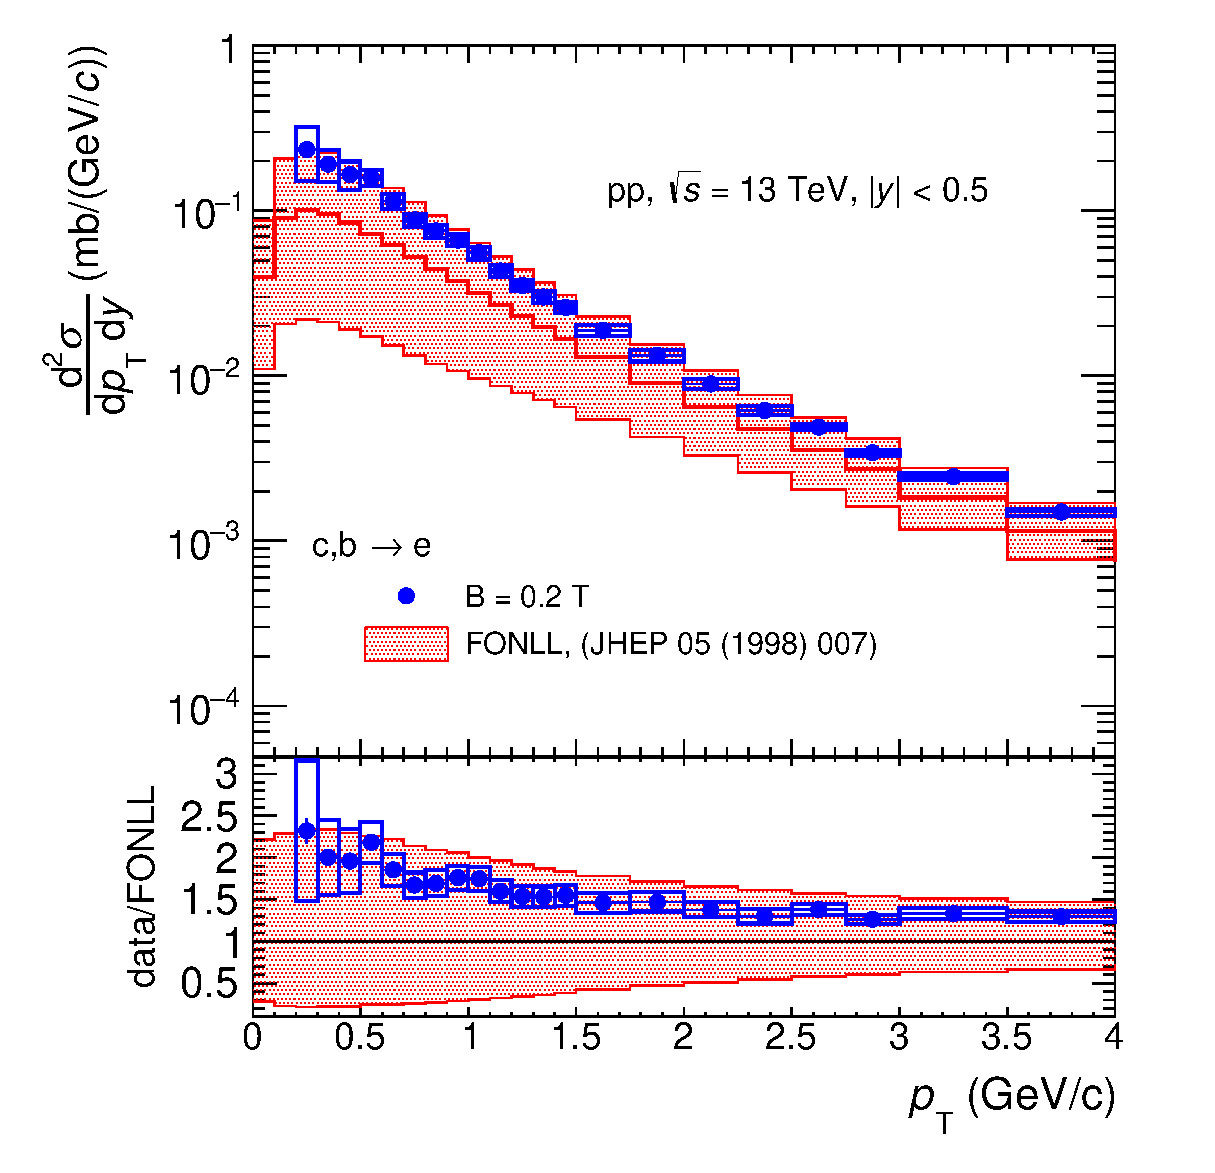
\includegraphics[scale = 0.3]{figurehttp://arxiv.org/abs/hep-ph/9803400s/Results/HFE_pp_LowB/HFE_comparison_05_lowB_with_FONLL_WSyst_Oct27_2020_UpEdgeKe3_CentralPointsHFE.eps}
\includegraphics[width=0.48\linewidth]{figures/Results/HFE_ppNormalB/HFE_Comparison_1.pdf}
\includegraphics[width=0.48\linewidth]{figures/Results/HFE_ppNormalB/Data_FONLL_HFE_1.pdf}
\caption{Left: In the upper panel, $p_{\rm T}$-differential cross section of electrons from heavy-flavour hadrons decays in pp collisions at $\sqrt{s} =$ 13 TeV measured at midrapidity with different detectors and datasets. In the bottom panel, ratios of the different measurements in the overlapping pt intervals. Right: In the upper panel, the $p_{\rm{T}}$ differential cross section is compared with FONLL predictions~\cite{Cacciari:1998it} and its ratio with respect to FONLL central value is shown in the bottom panel. Vertical bars and boxes denote statistical and systematical uncertainties, respectively.}        
\label{Fig:ppHFESpectra}
\end{figure}

\begin{figure}[!ht]
\centering
\includegraphics[width=0.5\linewidth]{figures/Results/HFE_pPb/HFE_InvariantCrossSection_pPb.pdf}
\caption{The $p_{\rm{T}}$ differential cross section of electrons from heavy-flavour hadron decays in \pPb collisions at \sqrtsNN = 8.16 TeV with TPC--TOF (blue data points) and TPC--EMCal (red data points).}        
\label{Fig:pPbHFESpectra}
\end{figure}

% Figure~\ref{Fig:ppHFESpectra} depicts the comparison of the cross section measured using using TPC--TOF (low and normal B) and TPC--EMCal detectors in the interval of xx-yy GeV$/c$. The cross sections are consistent with each other within the statistical and systematic uncertainties. The cross sections obtained with MB triggered sample (using TPC--EMCal) and EMCal triggered samples, EG2 and EG1, are also compared in the interval xx-yy GeV$/c$ and xx-yy GeV$/c$, respectively and are consistent within the uncertainties. 

 The $p_{\rm{T}}$-differential production cross section of electrons from semileptonic heavy-flavour hadron decays at midrapidity in \pPb collisions at $\sqrt{s_{\rm{NN}}} = 8.16$ TeV measured in the transverse momentum region $0.5 < p_{\rm{T}} < 26$~GeV$/c$ is shown in Fig.~\ref{Fig:pPbHFESpectra}. The statistical errors are presented as horizontal lines, the total systematic uncertainties are represented by the rectangular box. The Fig.~\ref{Fig:pPbHFESpectra} also presents the comparison of the cross section measured using using TPC--TOF and TPC--EMCal detectors in the interval of 3.0--4.0 GeV$/c$. The ratio of the cross-section measured using different detectors in the overlapping \pt range is presented in the bottom panel of the figure. The cross sections are consistent with each other within the statistical and systematic uncertainties. The cross sections obtained with MB triggered sample (using TPC--EMCal) and EMCal triggered sample, EG2 and EG1, are also compared in the interval  6.0--10.0 GeV$/c$ and 10.0--14.0 GeV$/c$, respectively, the ratio of which are presented in the bottom panel of the figure, and are consistent within the uncertainties. 

The nuclear modification factor, $R_{\rm{pPb}}$, requires a reference cross section for pp collisions at the same centre-of-mass energy. This was obtained by a $\sqrt{s}$-scaling procedure using pQCD calculations. The $p_{\rm{T}}$-dependent scaling factor was obtained by calculating the ratio of the production cross sections of electrons from heavy-flavour hadron decays from fixed order with next-to-leading-log (FONLL) calculations~\cite{Cacciari:1998it,Cacciari:2001td, Cacciari:2012ny} at $\sqrt{s}=13$ TeV to $\sqrt{s}=8.16$ TeV. The systematic uncertainty on the pp reference includes the systematic uncertainties on the measured cross section at $\sqrt{s}=13$ TeV, which is described above, and the $p_{\rm{T}}$-dependent scaling factor. The uncertainty on the scale factor ranges between 11--1\% and includes the uncertainties on the Parton Distribution Functions, quark masses, and factorisation and renormalization scales, as described in~\cite{Averbeck:2011ga}. The two contributions are added in quadrature leading to a total systematic of  $15–5\%$, depending on $p_{\rm{T}}$. In addition, a global normalization systematic uncertainty of 5\% from the pp analysis at $\sqrt{s}=13$ TeV was also considered. Figure ~\ref{Fig:HFESpectraComparison} shows the comparison of the $\sqrt{s}$-scaled  production cross sections of electron from heavy-flavour hadron decays in pp collisions at \sqrts = 13 TeV using aforementioned procedure with the production cross sections of electron from heavy-flavour hadron decays in \pPb collisions at \sqrtsNN = 8.16 TeV.

\subsection{Nuclear modification factor of electrons from heavy-flavour hadron decays in \pPb collisions}
The nuclear modification factor, $R_{\rm{pPb}}$, of electrons from heavy-flavour hadron decays as a function of transverse momentum at $\sqrt{s_{\rm{NN}}} = 8.16$ TeV is presented in Fig.~\ref{Fig:RpPb}. The statistical and systematic uncertainties of the spectra in p–Pb and pp collisions were propagated as uncorrelated. The normalization uncertainties are shown as a solid box at $R_{\rm{pPb}} = 1$. The $R_{\rm{pPb}}$ is consistent with unity within statistical and systematic uncertainties over the whole $p_{\rm{T}}$ range of the
measurement. Thus, the measurements are consistent with no modification over the measured $p_{\rm{T}}$ range. The sample of electrons from heavy-flavor hadron decays is dominated by beauty-hadron decays for $p_{\rm{T}} > 5$ GeV$/c$~\cite{Abelev:2012sca, Abelev:2014hla}. The $R_{\rm{pPb}}$ of unity indicates that the beauty production is not modified in \pPb collisions within the kinematic range of this measurement, which is also consistent with the measurement of $R_{\rm{pPb}}$ of beauty-decay electrons upto $p_{\rm{T}} = 8$ GeV$/c$ at $\sqrt{s_{\rm{NN}}} = 5.02$ TeV~\cite{Adam:2016wyz}. 

\begin{figure}[!ht]
\centering
\includegraphics[width=0.5\linewidth]{figures/Results/HFE_pPb/ppScaledReference.pdf}
\caption{The $p_{\rm{T}}$ differential cross section of electrons from heavy-flavour hadron decays in \pPb collisions at \sqrtsNN = 8.16 TeV compared with pp at \sqrts = 13 TeV scaled reference.}        
\label{Fig:HFESpectraComparison}
\end{figure}

\begin{figure}[!ht]
      \begin{center}
      \includegraphics[width=0.48\linewidth]{figures/Results/HFE_pPb/RpPb_8TeV.pdf}
      \includegraphics[width=0.48\linewidth]{figures/Results/HFE_pPb/RpPb_8TeV_ComparedWith5TeV.pdf}
      \end{center}
\caption{The nuclear modification factor ($R_{\rm{pPb}}$) of electrons from heavy-flavour hadron decays in \pPb collisions at \sqrtsNN = 8.16 TeV (left) and the $R_{\rm{pPb}}$ at \sqrtsNN = 8.16 TeV is compared with that at \sqrtsNN = 5.02 TeV and theoretical models at \sqrtsNN = 5.02 TeV (right).}    
\label{Fig:RpPb}
\end{figure}

\subsection[Self-normalized yield of electrons from heavy-flavour decays vs. normalized multiplicity]{Self-normalized yield of electrons from heavy-flavour decays vs. normalized multiplicity in pp and \pPb collisions}
The yield of electrons from heavy-flavour hadron decays was measured as described above in multiplicity intervals, and its ratio in a given multiplicity interval relative to the minimum bias yield is computed. The normalized yield of electrons from heavy-flavour decays, $\dndeta/\left<\dndeta\right>$, as a function of normalized charged-particle pseudorapidity density at midrapidity, $\dnchdeta/\left<\dnchdeta\right>$, is presented in Fig.~\ref{Fig:SelfnormalizedYield} in pp collisions at $\sqrt{s} =$ 13 TeV and in \pPb collisions at $\sqrt{s_{NN}}$ $=$ 8.16 TeV.  The results are normalized to INEL$>0$ event class. The measurements were performed in five $p_{\rm T}$ intervals from 0.5--30 GeV$/c$ for pp collisions and from 0.5--26 GeV$/c$ for \pPb collisions. The dashed line shown in the figure is a linear function with a slope of unity. The normalized yield allows us to examine events with a multiplicity more than 6 times (4 times) larger than the average multiplicity in pp (\pPb) collisions. In both pp and \pPb collisions, the normalized heavy-flavour decay electron yield grows faster than linear with the normalized multiplicity. This measurement is similar to the trend observed for inclusive charged-particle production~\cite{Acharya:2019mzb}, strange hadrons~\cite{Acharya:2019kyh}, D-mesons~\cite{Adam:2015ota,Adam:2016mkz},  J/$\psi$~\cite{Acharya:2020pit,Abelev:2012rz,Acharya:2020giw} and $\Upsilon$ mesons~\cite{Chatrchyan:2013nza}.
The bottom panel of Fig.~\ref{Fig:SelfnormalizedYield} shows the double ratio of the normalized heavy-flavour decay electron yield to the normalized multiplicity. It can be observed that for both pp and \pPb collisions the double ratio increases with multiplicity. In \pPb collisions, the increase is stronger for events with small multiplicity and slightly weaker increase at high multiplicity, and no dependence on \pt is observed. In pp collisions, while a strong increase is observed at low multiplicities for all \pt, the increase is weaker for low \pt electrons and a strong increase is seen for high \pt particles at higher multiplicities. The double ratio was fit with a linear function, as shown in Fig.~\ref{Fig:SNY_Ratio_pp} (right), and found to reasonable describe the data for all \pt bins. This indicates that in the measured \pt range the yield increases approx. with the square of the multiplicity with a coefficient which increases with \pt.

The measurement in pp collisions in intervals of $\pt$ shows that high $\pt$ heavy-flavour decay electron yield increases faster than the charged-particle multiplicity, while the
increase is smaller when we consider lower-$\pt$ particles. The yield increase is approximately a factor of 9 for the lowest measured $\pt$ ($0.5 < \pt < 1.5$ GeV$/c$) and a factor of 32 for the highest measured $\pt$ ($20 < \pt < 35$ GeV$/c$) for multiplicities of 6 times the average multiplicity. In the left panel of Fig.~\ref{Fig:SNY_Ratio_pp} the ratios of the average of the heavy-flavour decay electron relative yields in various \pt
intervals with respect to the $6 < \pt < 12$ GeV$/c$ interval values is shown. The yield of lower $\pt$ electrons is higher in low  multiplicity events, while it reduces in higher multiplicity events. Electrons at higher $\pt$ has an opposite trend, where the yield is lower in low  multiplicity events and increases at higher multiplicity. It should be noted that the contribution of heavy-flavour decay electrons from beauty hadron decays increases with $\pt$ and dominates over charm hadron decays for $\pt > 5-6$ GeV$/c$.  The observed $\pt$ dependence could be attributed to several effects - the momentum dependence of jet fragmentation affecting the measured multiplicity at midrapidity, and the momentum dependence of the fraction of electrons from charm and beauty hadron decays. 


\begin{figure}[!ht]
\includegraphics[width=0.46\linewidth]{figures/Results/HFE_ppNormalB/SNY_diagonal.pdf}
\hfil
\includegraphics[width=0.46\linewidth]{figures/Results/HFE_pPb/HFESelfNormalieYieldFullpT.pdf}
\caption{Self-normalized yield of electrons from heavy-flavour decays as a function of normalized charged-particle pseudorapidity density at midrapidity computed in \pp collisions at \sqrts = 13 TeV (left) and in \pPb collisions at \sqrtsNN = 8.16 TeV (right) in different \pt intervals.}
\label{Fig:SelfnormalizedYield}
\end{figure}

\begin{figure}[!h]
%\centering
%\includegraphics[width=0.6\linewidth]{figures/Results/HFE_ppNormalB/SNY_diagonal.pdf}
\includegraphics[width=0.48\linewidth]{figures/Results/HFE_ppNormalB/SNY_Pt_Ratio_0.pdf}
\includegraphics[width=0.48\linewidth]{figures/Results/HFE_ppNormalB/SNY_Fit_Diagonal_Linear.pdf}
\caption{ Ratio of the  normalized yield
in different \pt intervals with respect to that of the $6 < \pt < 12~{\rm GeV}/c$ interval (left) and double ratio of the normalized yield of heavy-flavour decay electrons to the normalized multiplicity in pp collisions at $\sqrts=13$ TeV (right) in three \pt ranges.}
\label{Fig:SNY_Ratio_pp}
\end{figure}

\begin{figure}[!h]
\centering
\includegraphics[width=0.5\linewidth]{figures/Results/HFE_ppNormalB/SNY_PYTHIA_0.pdf}
%\includegraphics[width=0.5\linewidth]{figures/Results/HFE_ppNormalB/SNY_PYTHIA_1.pdf}
\caption{Comparison of self-normalized yield of electrons from heavy-flavour decays computed in \pp collisions at \sqrts = 13 TeV for different \pt intervals with PYTHIA 8.2 calculations.}
     \label{Fig:SelfnormalizedYield_pp_PYTHIA}
\end{figure}

\begin{figure}[!h]
\centering
\includegraphics[width=0.45\linewidth]{figures/Results/HFE_ppNormalB/SNY_JPsi_PYTHIA_0.pdf}
\includegraphics[width=0.45\linewidth]{figures/Results/HFE_ppNormalB/SNY_ChargedParticles_High_6_10.pdf}
\includegraphics[width=0.45\linewidth]{figures/Results/HFE_ppNormalB/SNY_Dmeson_0.pdf}
\caption{Comparison of self-normalized yield of electrons from heavy-flavour decays computed in \pp collisions at \sqrts = 13 TeV  with the self-normalized yield of J/$\psi$ in \pp collisions at \sqrts = 13 TeV (top left), charged particles in \pp collisions at \sqrts = 13 TeV (top right) and with D-mesons in \pp collisions at \sqrts = 7 TeV (bottom), in \pt similar \pt bins.}
     \label{Fig:SNY_CompOtherPart_pp}
\end{figure}


%Compairson with pythia
The self-normalized yield of electrons from heavy-flavour hadron decays are compared with PYTHIA 8.2 simulations~\cite{Sjostrand:2014zea} in three \pt bins, as shown in Fig.~\ref{Fig:SelfnormalizedYield_pp_PYTHIA}. In PYTHIA 8.2 event generator multiparton interactions (MPI) and color reconnection (CR) mechanism are implemented,  which reproduces the charged-particle multiplicity distribution measured at LHC reasonably well ~\cite{Adam:2016mkz,Weber:2017kjj}. These mechanisms are important in order to describe the stronger than linear scaling of charm and beauty production with multiplicity as demonstrated in ~\cite{Adam:2015ota}. PYTHIA 8.2 reproduces well the overall trend in data. While PYTHIA describes the multiplicity dependence well at low \pt, the overall slope of the trend is overestimated at high \pt. A similar description of the \pt trend by PYTHIA is observed for charged particles~\cite{Acharya:2019mzb} in pp collisions at 13 TeV.   

The normalized heavy-flavour decay electron yield in pp collisions is compared with the normalized yield of J/$\psi$~\cite{Acharya:2020pit}, charged particles~\cite{Acharya:2019mzb} in pp collisions at 13 TeV, and with D-mesons~\cite{Adam:2015ota} in pp collisions at 7 TeV in Fig. ~\ref{Fig:SNY_CompOtherPart_pp}. A comparison of the PYTHIA predictions for J/$\psi$ and heavy-flavour decay electron yield has also been shown along with that of data in the figure (top left). The \pt range of electrons are selected to be similar to the measured \pt range of the compared particles. The slope of the increase of the normalized yield of electrons from heavy-flavour hadron decays as a function of normalized multiplicity is similar to that measured for J/$\psi$, charged particles and D-mesons in similar \pt ranges.
%The normalized yield of electrons from heavy-flavour hadron decays as a function of normalized multiplicity shows a similar trend as J/$\psi$, charged particles and D-mesons. 

In \pPb collisions the measurements in intervals of $\pt$ shows a weak $\pt$ dependence within the uncertainties of the measurement. The yield increase is approximately a factor of 7 for multiplicities of 4 times the average multiplicity. A quantitative comparison of the measurement in pp and \pPb collisions is not straight forward.  While the multiplicity
is measured for both pp and p–Pb collisions in the same pseudorapidity range in the laboratory system, it corresponds to different ranges in the centre-of-mass frame of the two collision systems, due to
the asymmetry of the beam energies in the p–Pb case. The multiplicity dependence of heavy-flavour production is also affected by the presence of multiple binary nucleon–nucleon interactions, and the initial conditions of the collision might be modified due to cold nuclear matter effects. 
The normalized heavy-flavour decay electron yield in \pPb collisions in different \pt ranges are compared with the normalized yield of D-mesons~\cite{Adam:2016mkz} in \pPb collisions at 5.02 TeV in Fig.~\ref{Fig:SNP_CompOtherPart_pPb}. Similar to the observation in pp collisions, the normalized yield of electrons from heavy-flavour hadron decays as a function of normalized multiplicity shows a similar trend as D-mesons.


The observed multiplicity dependence of heavy-flavour yield could be influenced by auto-correlation effects, where the measured multiplicity has contributions from particles arising from the fragmentation of partons produced in hard-scattering processes. However, measurements of normalized D-mesons~\cite{Adam:2015ota} and J/$\psi$~\cite{Acharya:2020pit} yield in pp collisions as a function of multiplicity measured at forward rapidity, with the aim to largely remove auto-correlation effects, also shows a significant faster than linear increase. Auto-correlation effects in the self-normalized yield of measurement of J/$\psi$ in pp collisions was studied using PYTHIA 8.2 simulations in ~\cite{Weber:2018ddv}. The study shows a weaker than linear increase of J/$\psi$ yield for multiplicities exceeding about three times the mean multiplicity in the absence of auto-correlation effects. The measurement of multiplicity dependence of J/$\psi$ in pp collisions at the LHC~\cite{Acharya:2020pit} can be described by several theoretical models that attribute the observed behavior to different underlying processes. PYTHIA 8.2 Monte-Carlo simulations and other theoretical models such as, models with the percolation mechanism~\cite{Ferreiro:2012fb}, higher Fock states in the proton~\cite{Kopeliovich:2013yfa}, effects from the colour glass condensate EFT~\cite{Ma:2018bax}, and multi-pomeron interaction combined with high-density effects (EPOS3 event generator~\cite{Werner:2013tya}) predict a faster than linear increase of J/$\psi$ yield as a function of multiplicity. All models predict an increase which is faster than linear, effectively as the result of a ($N_{\rm{ch}}-$dependent) reduction of the charged-particle multiplicity, realized through different physics mechanisms in the various approaches (color string reconnection or
percolation, gluon saturation, coherent particle production, 3-gluon fusion in gluon ladders/Pomerons)~\cite{Acharya:2020pit}.


\begin{figure}[!ht]
\centering
\includegraphics[width=0.6\linewidth]{figures/Results/HFE_pPb/2018-May-09-HFECompWithDMeson_pPb8TeV.pdf}
\caption{Self-normalized yield of electrons from heavy-flavour decays computed in \pPb collisions at \sqrtsNN = 8.16 TeV for different \pt intervals compared with self-normalized yield of average D meson in \pPb collisions at \sqrtsNN = 5.02 TeV .}
      \label{Fig:SNP_CompOtherPart_pPb}
\end{figure}

%%%%%%%%%%%%%%%%%%%%%%%%%%%%%%

%\begin{figure}[!ht]
%\centering
%\includegraphics[width=0.5\linewidth]{figures/Results/HFE_ppNormalB/SNY_Fit_Diagonal_Linear.pdf}
%\includegraphics[width=0.5\linewidth]{figures/Results/HFE_ppNormalB/SNY_Fit_Diagonal_Power.pdf}
%\caption{Fit to double Ratio. {\bf The Chi2/NDF value is better for power law fit than linear for the lowest and highest  bins (red and green).  Chi2/NDF for blue is better with linear. We can check and try to find a trend, how the double ratio fits better with some function and  changes from linear and then to some other function.} The green fit doesnot look to be good with either, I have to find a function that fits the green plot better. I will do more fits and update these plots}
   %   \label{Fig:SelfnormalizedYield_Fit}
%\end{figure}


%\begin{figure}[!ht]
%\centering
%\includegraphics[width=0.5\linewidth]{figures/Results/HFE_ppNormalB/SNY_PYTHIA_Only_0.pdf}
%\includegraphics[width=0.5\linewidth]{figures/Results/HFE_ppNormalB/SNY_PYTHIA_DBe_0.pdf}
%\caption{{\bf For mow I have kept both, I removed one}Comparison of self-normalized yield of electrons from heavy-flavour decays computed in \pp collisions at \sqrts = 13 TeV for different \pt intervals with PYTHIA8.2 prediction (b,c to e separately).}
%\label{Fig:SelfnormalizedYield_pp_PYTHIA}
%\end{figure}


%\begin{figure}[!ht]
%\centering
%\includegraphics[width=0.5\linewidth]{figures/Results/HFE_ppNormalB/SNY_Dmeson_0.pdf}
%\caption{Comparison of self-normalized yield of electrons from heavy-flavour decays computed in \pp collisions at \sqrts = 13 TeV for lowest  \pt intervals with Dmeson at 7 TeV [1505.00664].}
 %    \label{Fig:SelfnormalizedYield_pp_Dmeson}
%\end{figure}

%\begin{figure}[!ht]
%\centering
%\includegraphics[width=0.5\linewidth]{figures/Results/HFE_ppNormalB/SNY_ChargedParticles_High_6_10.pdf}
%\caption{Comparison of self-normalized yield of electrons from heavy-flavour decays computed in \pp collisions at \sqrts = 13 TeV for lowest  \pt intervals with charged particles  at 13 TeV [1905.07208].}
 %    \label{Fig:SelfnormalizedYield_pp_ChergedParticle}
%\end{figure}


%\begin{figure}[!ht]
%\centering
%\includegraphics[width=0.6\linewidth]{figures/Results/HFE_pPb/ALICE_SNHFE.pdf}
%\caption{Self-normalized yield of electrons from heavy-flavour decays computed in \pPb collisions at \sqrtsNN = 8.16 TeV for different \pt intervals.}
 %     \label{Fig:SelfnormalizedYield_pPb}
%\end{figure}

%\subsection{Comparison with other results}\label{section:ResultComparison}



%\subsection{Comparison with theoretical predictions}\label{section:comparisonToModels}





\section{Summary}\label{section:summary}
Heavy-flavour production at midrapidity was studied using electrons from heavy-flavour hadron decays in pp collisions at $\sqrt{s}=13$ TeV and in \pPb collisions at \sqrtsNN=8.16 TeV with the ALICE detector at the LHC. The \pt differential production cross-section of electrons from heavy-flavour hadron decays in pp collisions was measured in the range of 0.2 $<p_{\rm T}<$ 35 GeV$/c$ and compared with Fixed-Order-Next-to-Leading-Log pQCD calculations.
%, which and shows a good agreement within the statistical and systematic uncertainties. 
{The data lies on the upper edge of the theoretical uncertainties.} The measurements in pp collisions are an important test of pQCD calculations at the highest energy measured. The \pt differential production cross-section of electrons from heavy-flavour hadron decays in \pPb collisions was measured in the range of 0.5 $<p_{\rm T}<$ 26 GeV$/c$. The nuclear modification factor in \pPb collisions, $R_{\rm{pPb}}$, was calculated and found to be consistent with unity within the statistical and systematic uncertainties. The $R_{\rm{pPb}}$ at \sqrtsNN = 8.16 TeV was also found to be consistent with that measured at \sqrtsNN = 5.02 TeV. The $R_{\rm{pPb}}$ results shows no hot-QCD effects in the measured \pt range and provides important inputs for cold nuclear matter calculations at \sqrtsNN = 8.16 TeV. 

The multiplicity dependent production of electrons from heavy-flavour hadron decays was measured using the self-normalized yield  as a function of normalized charged particle pseudorapidity density at midrapidity in pp and \pPb collisions as a function of transverse momentum. A faster than linear growth was observed in both pp and p--Pb collisions, similar to the observation for inclusive charged particles and several other charm and beauty hadrons. While in p-Pb collisions no \pt dependence is observed within uncertainties, in pp collisions a strong \pt dependence is seen with high \pt electrons showing a faster increase as a function of normalized multiplicity. The measurement of self-normalized yield of electrons from heavy-flavour hadron decays in pp collisions was compared with PYTHIA 8.2 simulations, which reproduces the trend qualitative, but overestimates the slope at high \pt. While strong conclusions are difficult to make due the contributions of jets from hard-scattering process to the measured multiplicity at midrapidity, the self-normalized yield measurements as a function of normalized multiplicities provides more insight into the production of heavy-flavour hadrons and its interplay with charged-particle production.  Disentangling the production of heavy-flavour hadrons and the charged particle multiplicity will be an important step towards shedding light on the mechanism of production and hadronization of charm and beauty quarks in high-multiplicity environment in pp and \pPb collisions. 



\clearpage
\section*{Acknowledgements}\label{section:acknowledgements}


\clearpage

\bibliographystyle{utphys}   % Remember we use title in the biblio
\bibliography{bibliography.bib}

%\bibliography{./bib/AlicePaper2016,./bib/ref_corrections,./bib/ref_d0reconstructionandselections,./bib/ref_datasampleandselection,./bib/ref_eventshapedefinitions,./bib/ref_experimentalsetup,./bib/ref_multiplicitydefinitions,./bib/ref_introduction,./bib/ref_systematics,biblio}


\end{document}
